\documentclass[conference]{IEEEtran}
\IEEEoverridecommandlockouts
\usepackage{cite}
\usepackage{amsmath,amssymb,amsfonts}
\usepackage{algorithmic}
\usepackage{graphicx}
\usepackage{textcomp}
\usepackage{xcolor}
\usepackage{booktabs}
\usepackage{multirow}
\def\BibTeX{{\rm B\kern-.05em{\sc i\kern-.025em b}\kern-.08em
    T\kern-.1667em\lower.7ex\hbox{E}\kern-.125emX}}

% Run gather_sweep_local_insights.py to generate report_generated.tex and plot_local/;
% if present, a short ``Exploratory partial run'' subsection is included.
\IfFileExists{report_generated.tex}{% Auto-generated by gather_sweep_local_insights.py -- do not edit by hand

\newcommand{\LocalBestWmapeVal}{0.0744}
\newcommand{\LocalBestRtwoVal}{0.9794}
\newcommand{\LocalBestWmapeTest}{0.0705}
\newcommand{\LocalBestRtwoTest}{0.9813}
\newcommand{\LocalRunPartial}{partial (incomplete)}
\newcommand{\LocalBestModel}{rfr}

% Comparison table rows (prior sweeps)
\newcommand{\PriorWmapeDim}{0.1968}
\newcommand{\PriorRtwoDim}{0.8846}
\newcommand{\PriorWmapeQual}{0.0723}
\newcommand{\PriorRtwoQual}{0.9807}
\newcommand{\PriorWmapeAll}{0.0695}
\newcommand{\PriorRtwoAll}{0.9812}
\gdef\IncludePartialRun{1}}{\newcommand{\LocalBestWmapeVal}{---}\newcommand{\LocalBestRtwoVal}{---}\newcommand{\LocalBestModel}{---}\newcommand{\LocalRunPartial}{N/A}}

\begin{document}

\title{Comparative Analysis of Regression Models for Diamond Price Prediction: A Feature-Set Sweep Study}

\author{\IEEEauthorblockN{1\textsuperscript{st} Raymond Pridgen}
\IEEEauthorblockA{\textit{Department of Computer Science} \\
\textit{Coastal Carolina University}\\
Conway, SC \\
rkpridgen@coastal.edu}
}

\maketitle

\begin{abstract}
This paper presents a systematic evaluation of three regression models---Random Forest (RFR), K-Nearest Neighbors (KNN), and ElasticNet---for predicting diamond prices from physical and qualitative attributes. We conduct 9,798 hyperparameter configurations across three feature-set sweeps: dimensional features only (x, y, z), quality features only (carat, cut, color, clarity, depth, table), and all nine features combined. We evaluate performance using weighted Mean Absolute Percentage Error (wMAPE), $R^2$, RMSE, and MAE. Our results demonstrate that Random Forest consistently outperforms competing models, achieving a best validation wMAPE of 0.0695 ($R^2=0.981$) with all features. A leave-one-out ablation analysis reveals that clarity and color---despite modest Gini importance---are the most irreplaceable features, while carat weight is largely redundant with physical dimensions. These findings highlight the importance of ablation-based importance metrics over split-count measures and confirm that nonlinear models are essential for capturing the complex pricing dynamics of gemstones.
\end{abstract}

\section{Introduction}

Diamond pricing is a complex function of physical and aesthetic attributes, traditionally summarized by the ``4Cs'': carat weight, cut quality, color grade, and clarity grade~\cite{b1}. While domain experts rely on grading standards and market experience, machine learning offers the potential for objective, data-driven price estimation. Accurate price prediction has practical applications in retail, insurance valuation, and investment analysis.

Prior work on diamond price prediction has explored linear regression~\cite{b2}, neural networks~\cite{b3}, and tree-based methods~\cite{b4}, generally finding that nonlinear models outperform linear ones. However, systematic comparisons across feature subsets---particularly the distinction between dimensional and qualitative attributes---remain underexplored.

In this study, we address three questions:
\begin{itemize}
\item How do physical dimensions alone compare to quality grades for price prediction?
\item Which model family (linear, instance-based, or tree-based) best captures diamond pricing dynamics?
\item Which features provide unique, irreplaceable information vs.\ redundant signal?
\end{itemize}

We conduct a comprehensive hyperparameter sweep across three model types and three feature sets, totaling 9,798 configurations, and complement standard metrics with leave-one-out ablation analysis to disentangle feature importance from feature redundancy.

\section{Dataset and Preprocessing}

\subsection{Dataset Description}
We use the classic Diamonds dataset~\cite{b5} containing 53,940 round-cut diamonds with ten attributes: a row identifier (\texttt{number}), four continuous measures (\texttt{carat}, \texttt{depth}, \texttt{table}, \texttt{price}), three physical dimensions (\texttt{x}, \texttt{y}, \texttt{z} in mm), and three categorical grades (\texttt{cut}, \texttt{color}, \texttt{clarity}). The target variable is \texttt{price} (USD), which ranges from \$326 to \$18,823 with a right-skewed distribution (mean \$3,933, median \$2,401).

\subsection{Feature Sets}
Three feature configurations were evaluated:
\begin{itemize}
\item \textbf{Dimensions} (3 features): \texttt{x}, \texttt{y}, \texttt{z}---physical measurements in millimeters.
\item \textbf{Qualities} (6 features): \texttt{carat}, \texttt{cut}, \texttt{color}, \texttt{clarity}, \texttt{depth}, \texttt{table}---weight and grading attributes.
\item \textbf{All Features} (9 features): the union of dimensions and qualities.
\end{itemize}

The \texttt{number} column (row index) was excluded from all experiments.

\subsection{Preprocessing Pipeline}
Data was shuffled with a fixed seed (42) and split 70/15/15 into train ($n=37,758$), validation ($n=8,091$), and test ($n=8,091$) sets. A scikit-learn \texttt{ColumnTransformer} pipeline applied median imputation and standard scaling to numeric features, and most-frequent imputation with one-hot encoding to categorical features (\texttt{cut}: 5 levels, \texttt{color}: 7 levels, \texttt{clarity}: 8 levels).

\section{Methodology}

\subsection{Model Types}
Three regression model families were evaluated:

\textbf{Random Forest Regressor (RFR)}~\cite{b6}: An ensemble of decision trees with bagging. Grid: \texttt{n\_estimators} $\in \{50, 100, 300, 800\}$, \texttt{max\_depth} $\in \{5, 10, 20, 30, \text{None}\}$, \texttt{min\_samples\_leaf} $\in \{1, 2, 4, 8, 16\}$.

\textbf{K-Nearest Neighbors (KNN)}: Instance-based learning using distance in the scaled feature space. Grid: \texttt{n\_neighbors} $\in \{2, 5, 10, 30\}$, \texttt{weights} $\in \{\text{uniform}, \text{distance}\}$.

\textbf{ElasticNet}~\cite{b7}: Regularized linear regression combining L1 and L2 penalties. Grid: \texttt{alpha} $\in \{0.1, 0.3, 0.5, 1.0, 1.5, 2.0\}$, \texttt{l1\_ratio} $\in \{0.1, 0.33, 0.66, 0.85, 1.0\}$.

\subsection{Evaluation Metrics}
Models were compared using:
\begin{itemize}
\item \textbf{wMAPE} (primary): $\frac{\sum |y_i - \hat{y}_i|}{\sum |y_i|}$, which weights errors proportional to actual values, avoiding the instability of standard MAPE for low-price items.
\item \textbf{$R^2$}: Coefficient of determination.
\item \textbf{RMSE}: Root mean squared error (USD).
\item \textbf{MAE}: Mean absolute error (USD).
\end{itemize}

All hyperparameter selection was performed on the validation set; the test set was used only for final reporting.

\subsection{Sweep Configuration}
Each sweep evaluated every model--hyperparameter--feature combination, with leave-one-out feature ablation enabled for the all-features sweep. Total configurations: 552 (dimensions) + 7,866 (qualities, including feature subsets) + 1,380 (all features, with ablation) = 9,798.

\section{Results}

\subsection{Overall Best Performance}

Table~\ref{tab:best_overall} presents the best-performing configuration from each sweep. Random Forest achieves the best results in all three sweeps.

\begin{table}[htbp]
\caption{Best Model per Sweep (by validation wMAPE)}
\begin{center}
\begin{tabular}{lccccc}
\toprule
\textbf{Feature Set} & \textbf{Model} & \textbf{wMAPE} & \textbf{$R^2$} & \textbf{RMSE} & \textbf{MAE} \\
\midrule
Dimensions (3) & RFR & 0.1968 & 0.885 & 1362.7 & 778.1 \\
Qualities (6) & RFR & 0.0723 & 0.981 & 557.1 & 285.9 \\
All Features (9) & RFR & \textbf{0.0695} & \textbf{0.981} & \textbf{552.0} & \textbf{274.7} \\
\bottomrule
\end{tabular}
\label{tab:best_overall}
\end{center}
\end{table}

Quality features reduce wMAPE by 63.2\% compared to dimensions alone (0.0723 vs.\ 0.1968). Adding dimensions to qualities yields a further 3.9\% relative reduction to 0.0695.

\subsection{Model Comparison Across Sweeps}

Fig.~\ref{fig:wmape_comparison} shows the best validation wMAPE for each model across all three feature sweeps. Table~\ref{tab:model_comparison} provides the complete comparison.

\begin{figure}[htbp]
\centerline{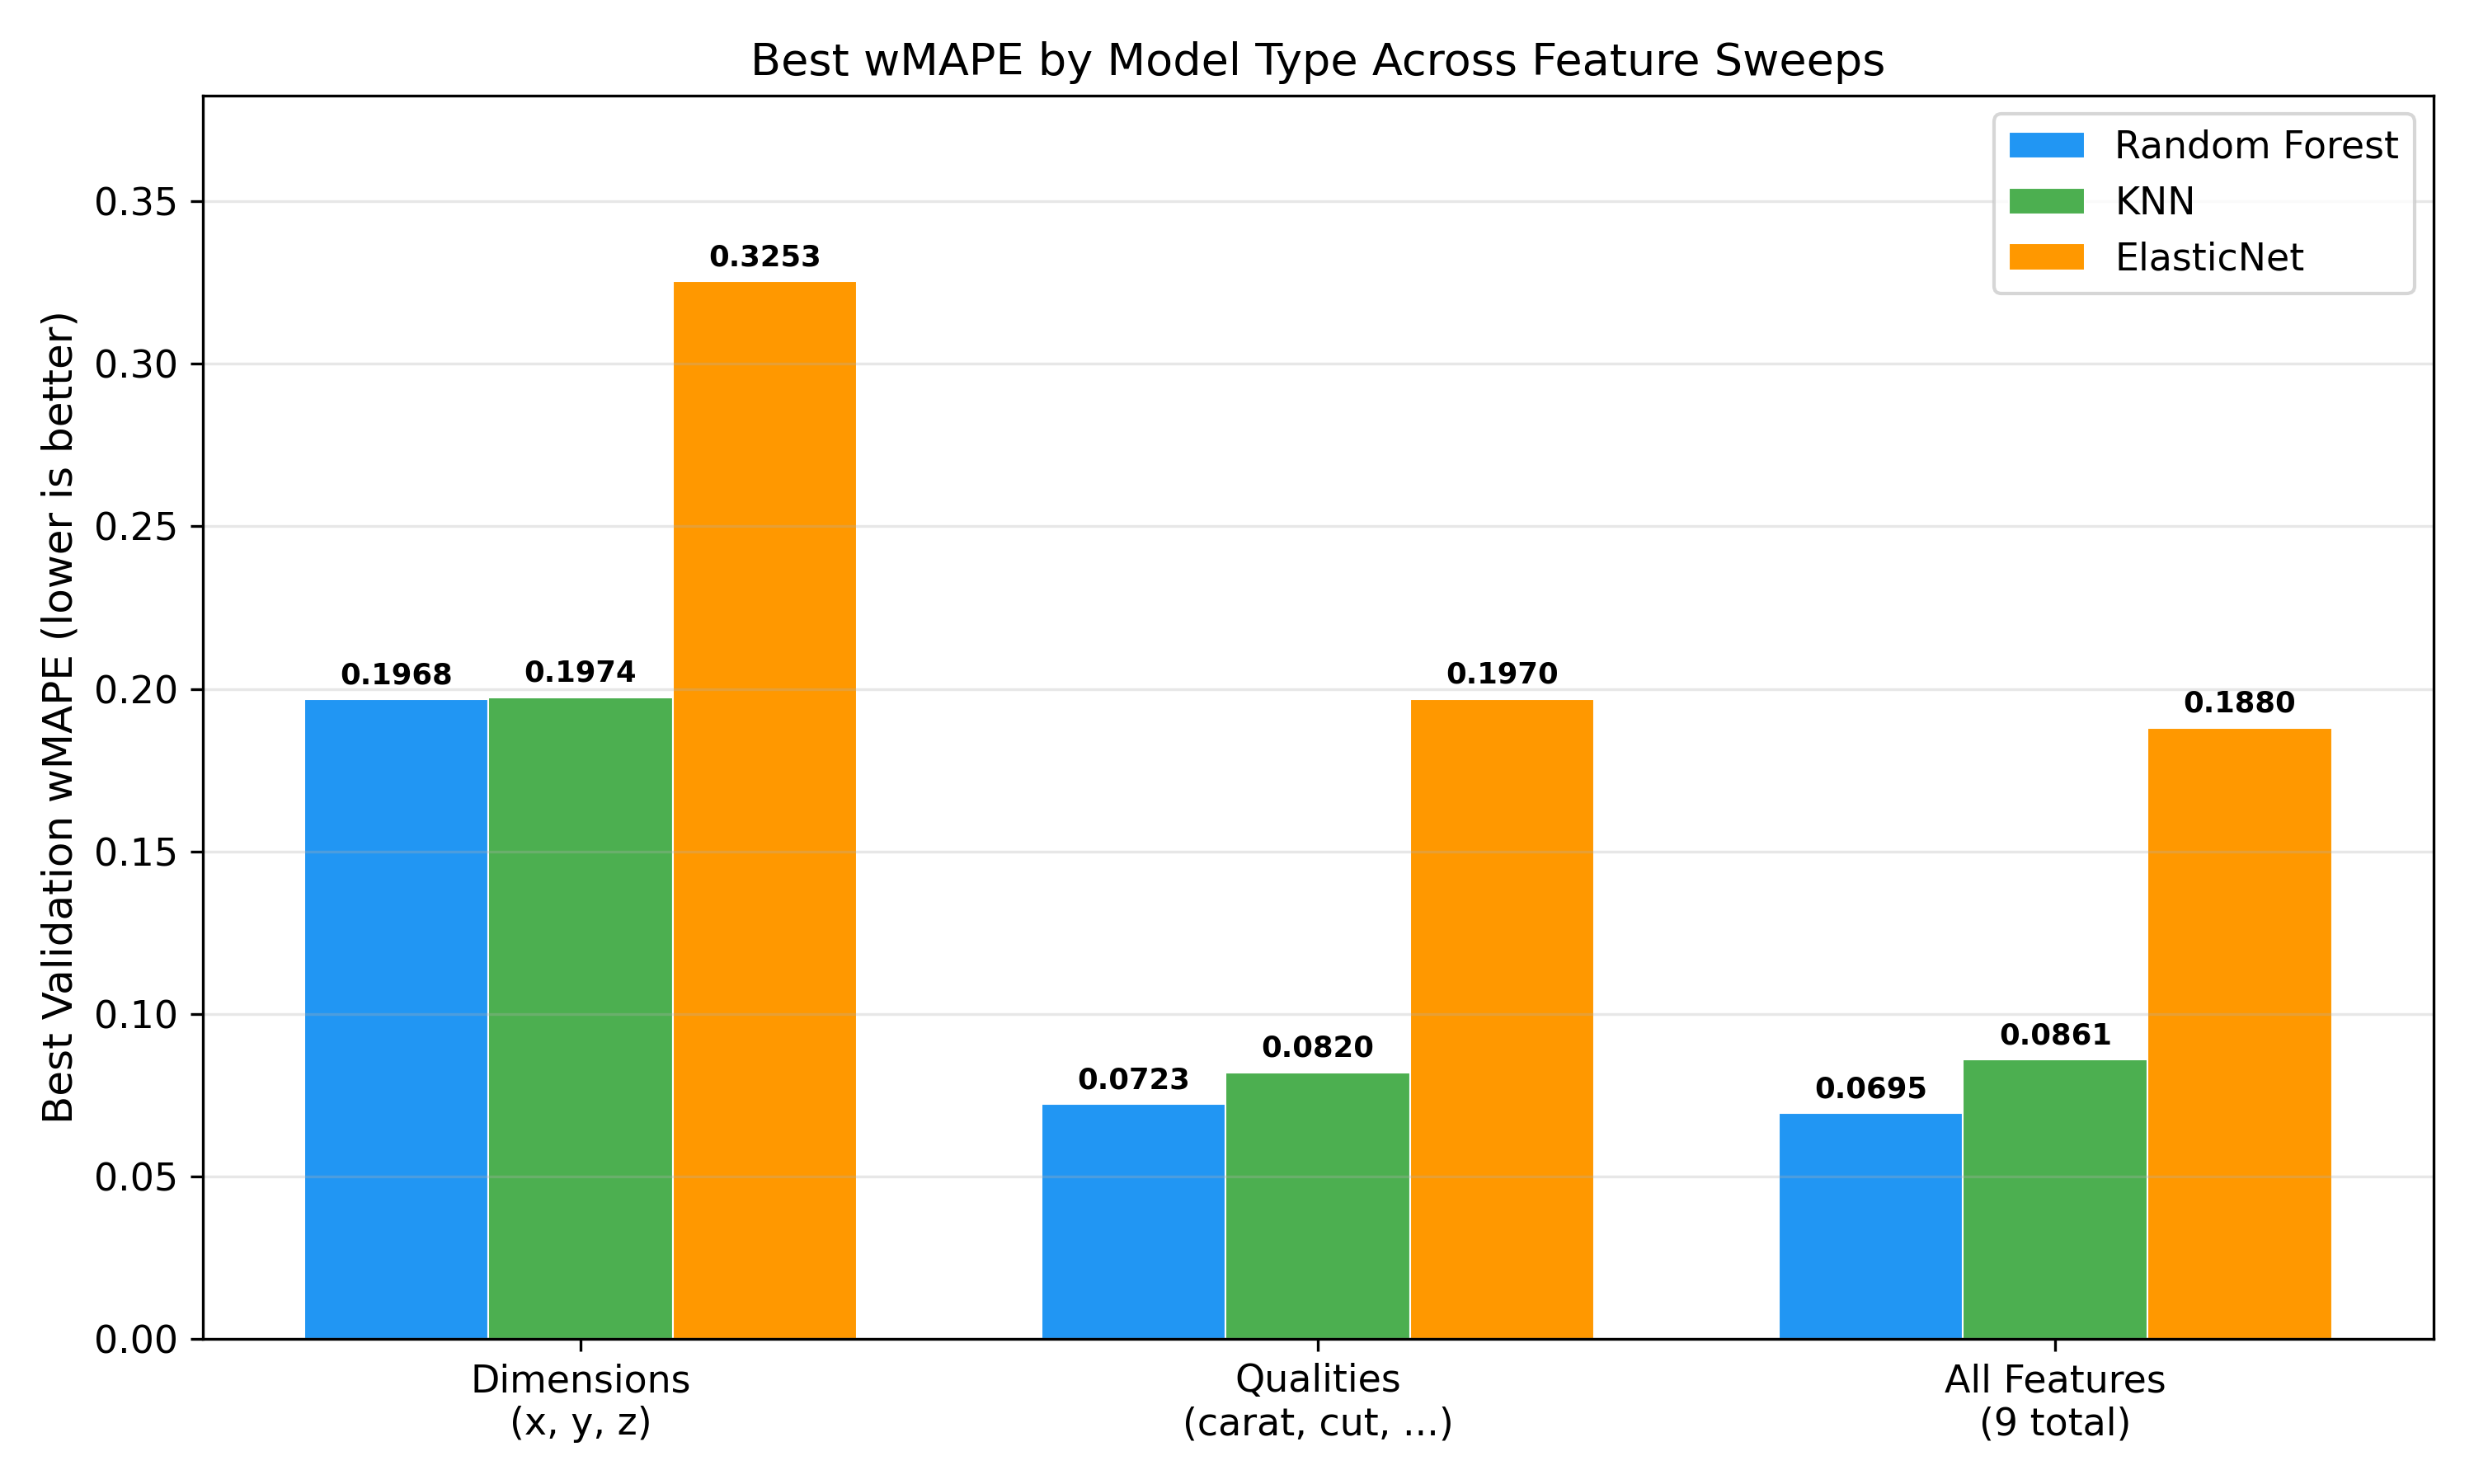
\includegraphics[width=\columnwidth]{plots/cross_sweep_wmape_comparison.png}}
\caption{Best validation wMAPE by model type and feature set. Random Forest achieves the lowest wMAPE in every configuration.}
\label{fig:wmape_comparison}
\end{figure}

\begin{figure}[htbp]
\centerline{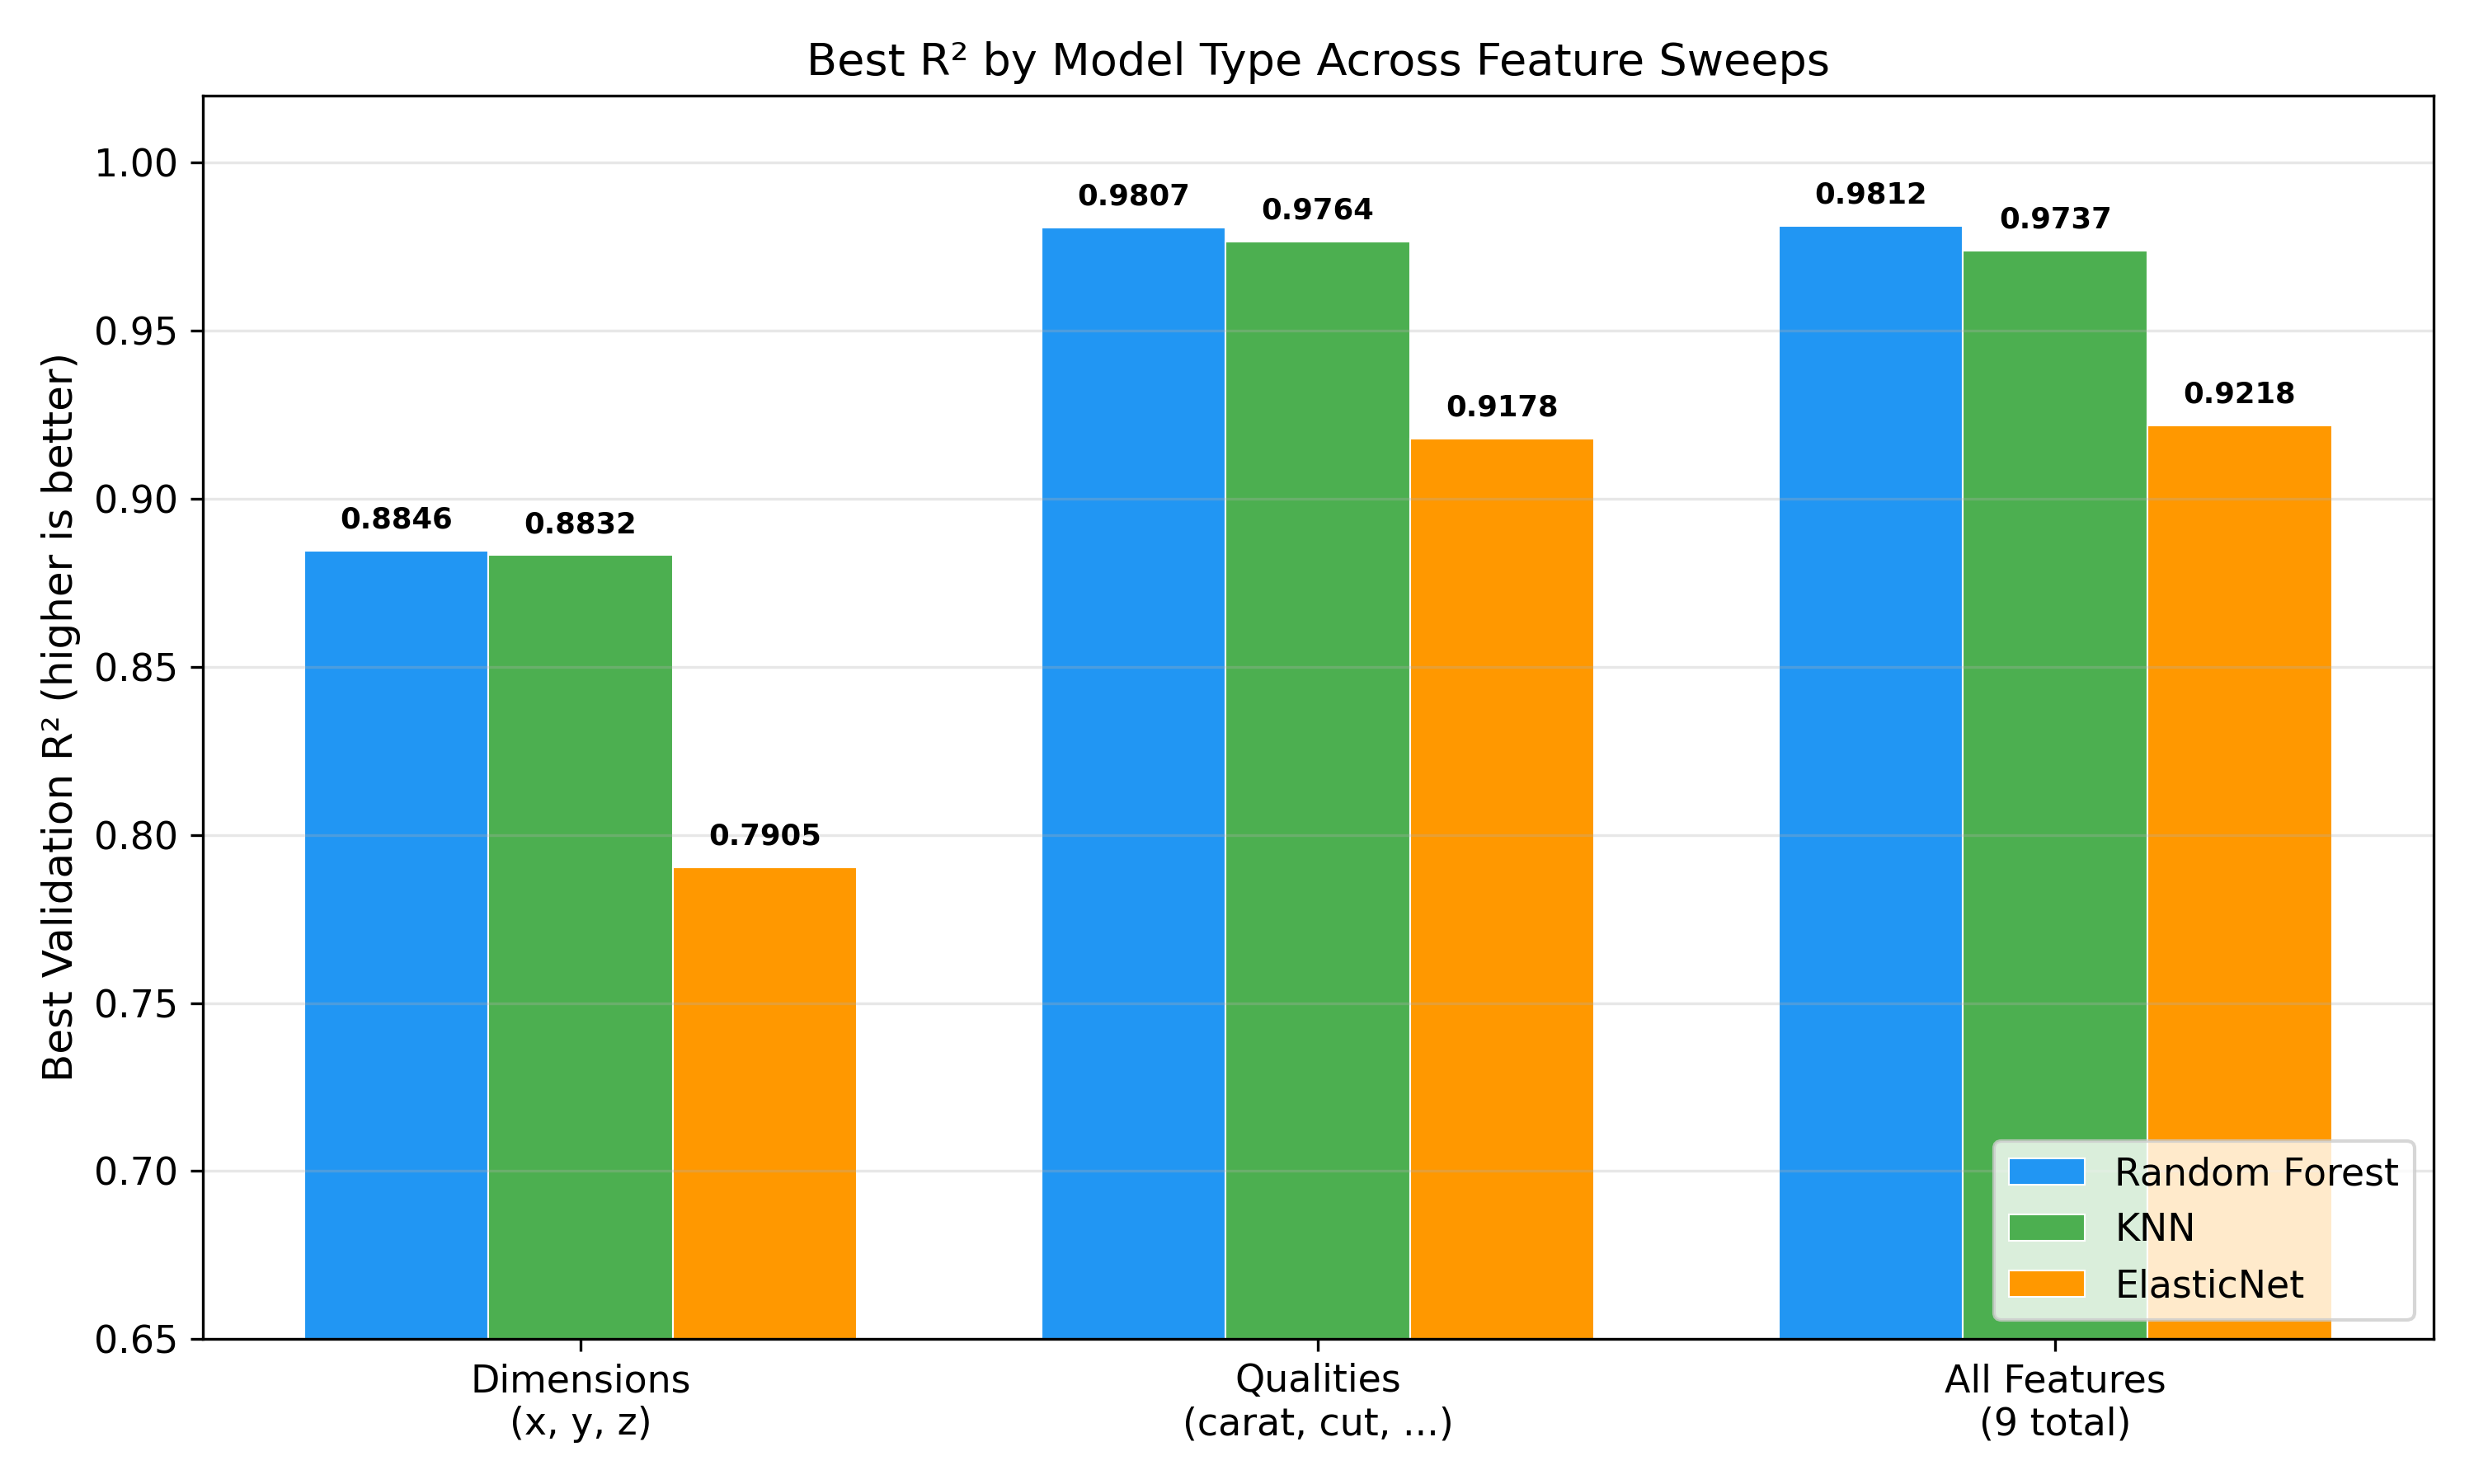
\includegraphics[width=\columnwidth]{plots/cross_sweep_r2_comparison.png}}
\caption{Best validation $R^2$ by model type and feature set. All models improve substantially from dimensions to qualities, with diminishing returns when adding dimensions to quality features.}
\label{fig:r2_comparison}
\end{figure}

\begin{table}[htbp]
\caption{Best Validation Metrics per Model Type and Sweep}
\begin{center}
\begin{tabular}{llcccc}
\toprule
\textbf{Sweep} & \textbf{Model} & \textbf{wMAPE} & \textbf{$R^2$} & \textbf{RMSE} & \textbf{MAE} \\
\midrule
\multirow{3}{*}{Dimensions} & RFR & 0.1968 & 0.885 & 1362.7 & 778.1 \\
 & KNN & 0.1974 & 0.883 & 1371.1 & 780.7 \\
 & ElasticNet & 0.3253 & 0.769 & 1926.3 & 1286.4 \\
\midrule
\multirow{3}{*}{Qualities} & RFR & 0.0723 & 0.981 & 557.1 & 285.9 \\
 & KNN & 0.0820 & 0.976 & 623.9 & 324.4 \\
 & ElasticNet & 0.1970 & 0.913 & 1183.2 & 778.8 \\
\midrule
\multirow{3}{*}{All Feat.} & RFR & 0.0695 & 0.981 & 552.0 & 274.7 \\
 & KNN & 0.0861 & 0.972 & 667.6 & 340.3 \\
 & ElasticNet & 0.1880 & 0.922 & 1122.3 & 743.5 \\
\bottomrule
\end{tabular}
\label{tab:model_comparison}
\end{center}
\end{table}

\subsection{wMAPE Distribution Analysis}

Fig.~\ref{fig:boxplots} shows the wMAPE distribution across all hyperparameter configurations for each model and sweep. The qualities and all-features sweeps exhibit much tighter distributions for RFR and KNN, indicating that these models are robust to hyperparameter choices when quality features are available.

\begin{figure}[htbp]
\centerline{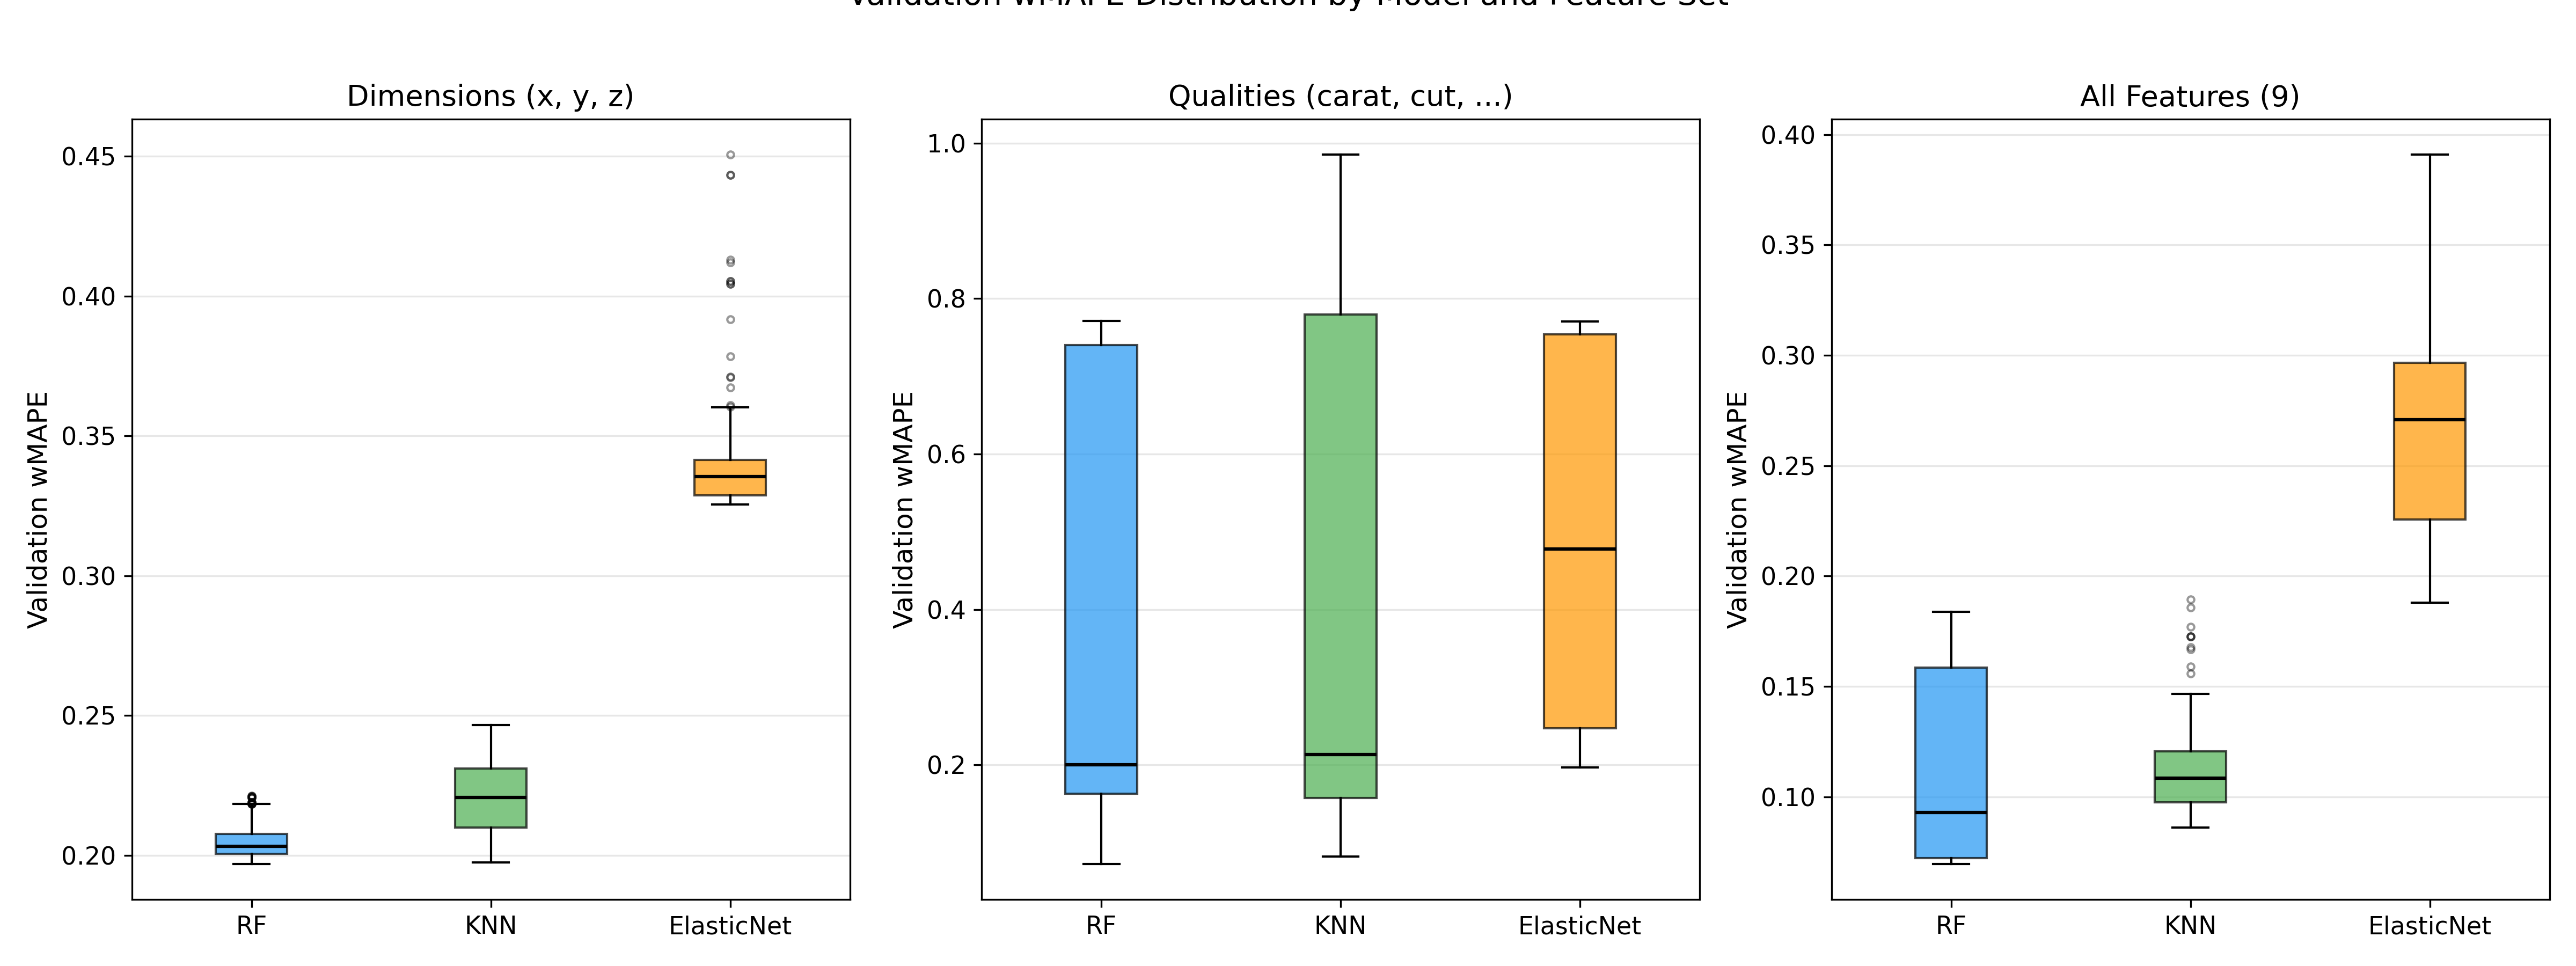
\includegraphics[width=\columnwidth]{plots/wmape_boxplots_by_sweep.png}}
\caption{Validation wMAPE distributions by model type and feature set. ElasticNet shows the highest variance, particularly in the qualities sweep where some feature subsets produce wMAPE $> 0.9$.}
\label{fig:boxplots}
\end{figure}

\ifdefined\IncludePartialRun
\subsection{Exploratory Partial Run (Local Sweep)}
An additional run was started with a 5-feature set (clarity, color, carat, $y$, $x$) and an extended RFR/KNN grid (e.g., more trees, deeper trees, more neighbors) to probe whether a focused subset could match the all-features sweep. The run is \LocalRunPartial\ (450/1560 combos completed). The best configuration so far is \LocalBestModel\ with validation wMAPE \LocalBestWmapeVal\ and $R^2$ = \LocalBestRtwoVal---competitive with the Qualities sweep but not surpassing the All-features best (0.0695 / 0.981). Fig.~\ref{fig:local_comparison} places this run in context; it does not alter the main conclusions above.
\begin{figure}[htbp]
\centerline{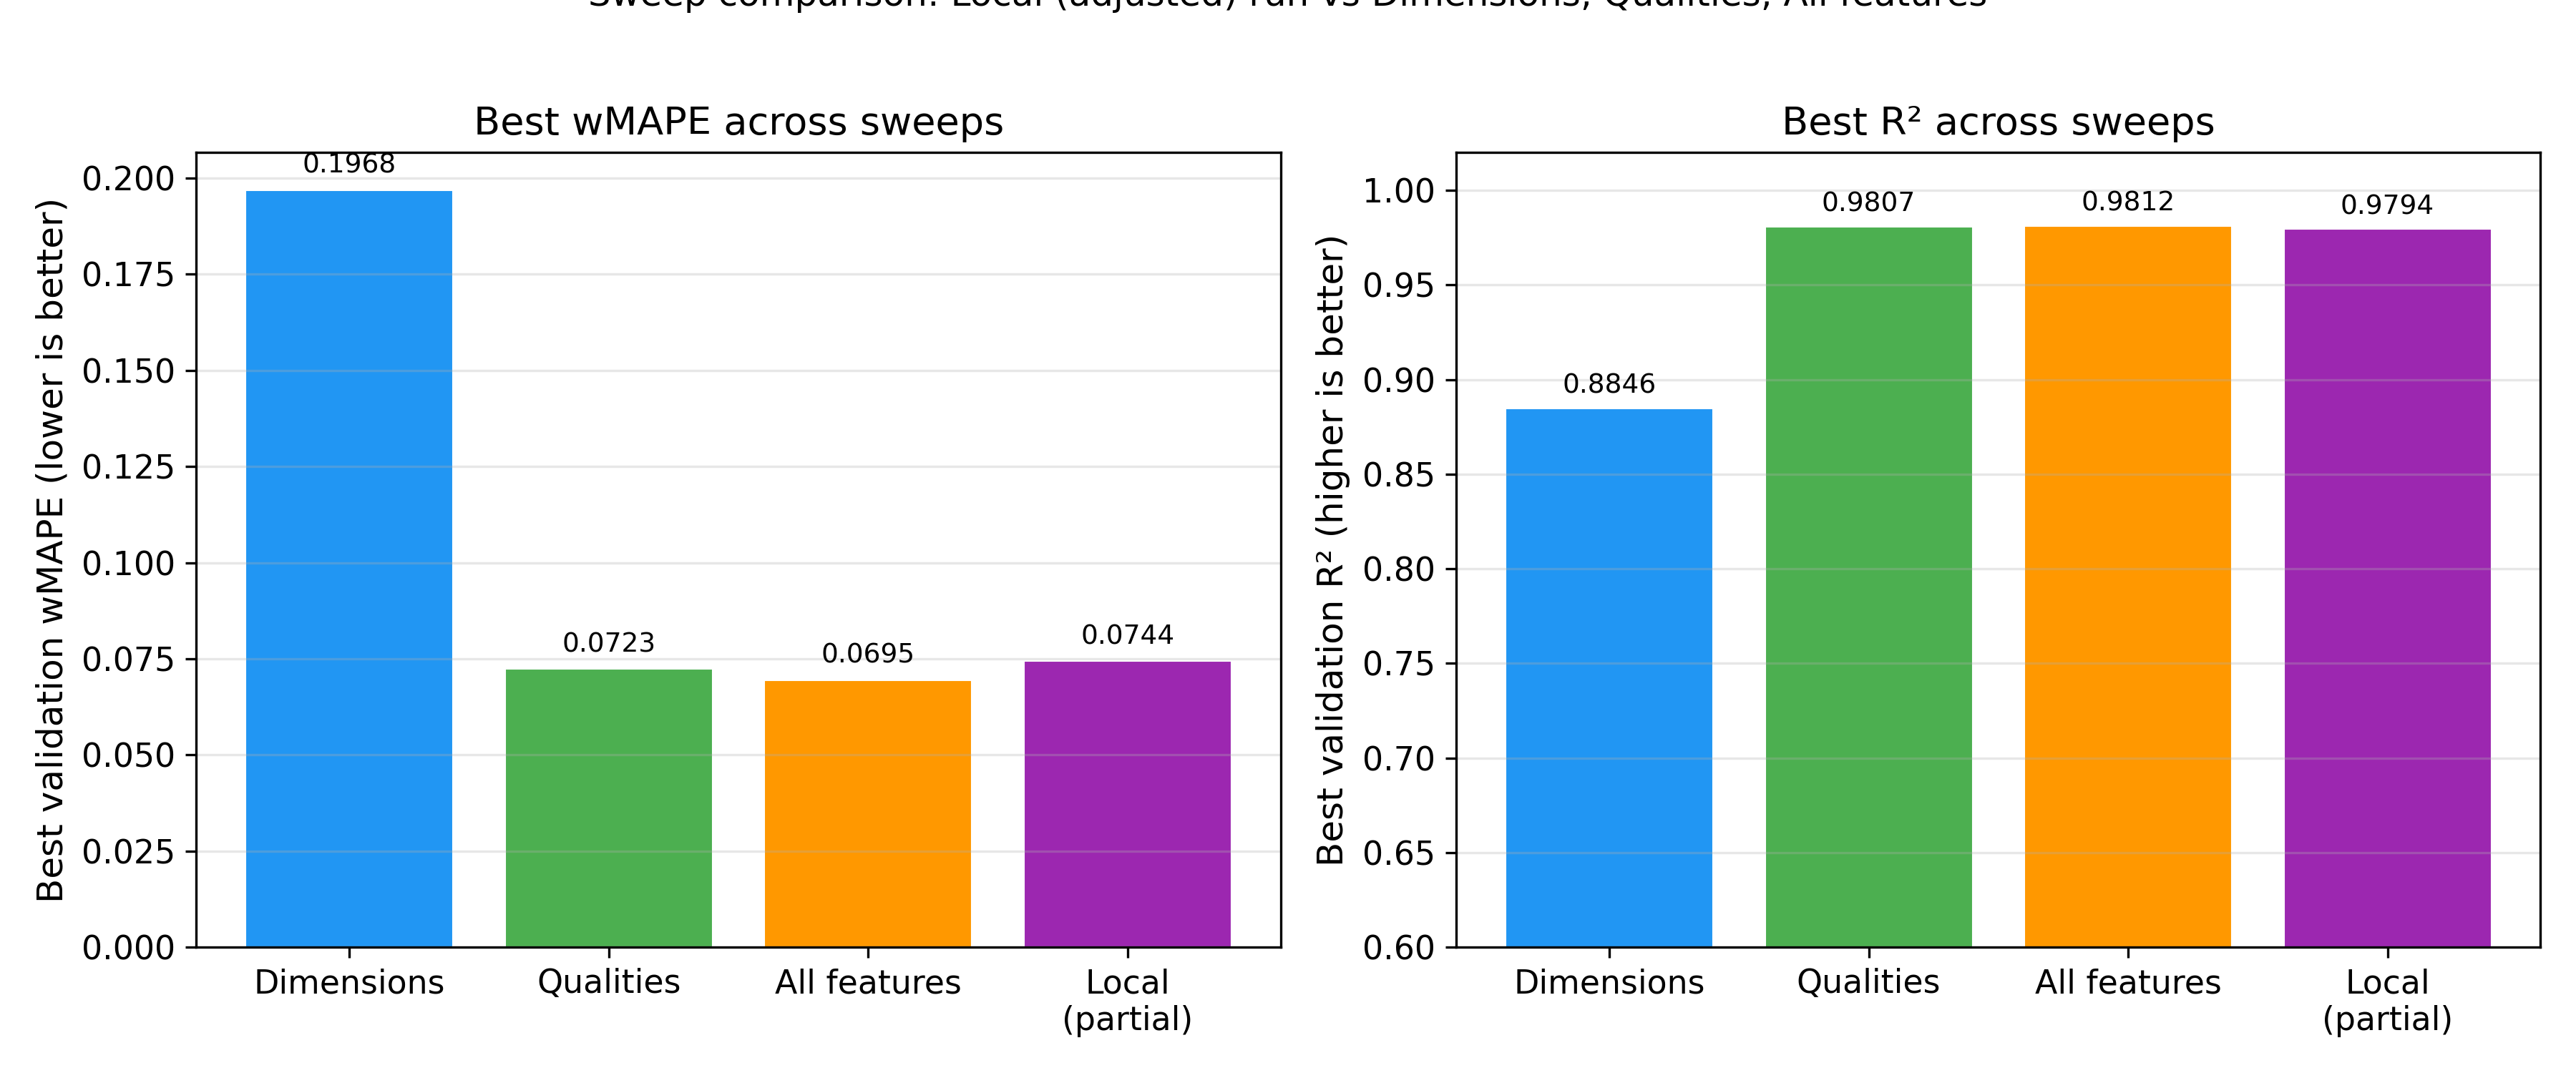
\includegraphics[width=\columnwidth]{plot_local/comparison_overall_wmape_r2.png}}
\caption{Best validation wMAPE and $R^2$ across the three full sweeps and the exploratory partial run (Local).}
\label{fig:local_comparison}
\end{figure}
\fi

\subsection{Random Forest Hyperparameter Analysis}

The Random Forest has three primary hyperparameters---\texttt{n\_estimators}, \texttt{max\_depth}, and \texttt{min\_samples\_leaf}---which interact to determine model capacity and regularization. We examine each pairwise interaction in detail.

\subsubsection{n\_estimators vs.\ max\_depth}

Fig.~\ref{fig:rf_heatmaps} shows RF performance heatmaps for \texttt{n\_estimators} vs.\ \texttt{max\_depth} across all three sweeps.

\begin{figure}[htbp]
\centerline{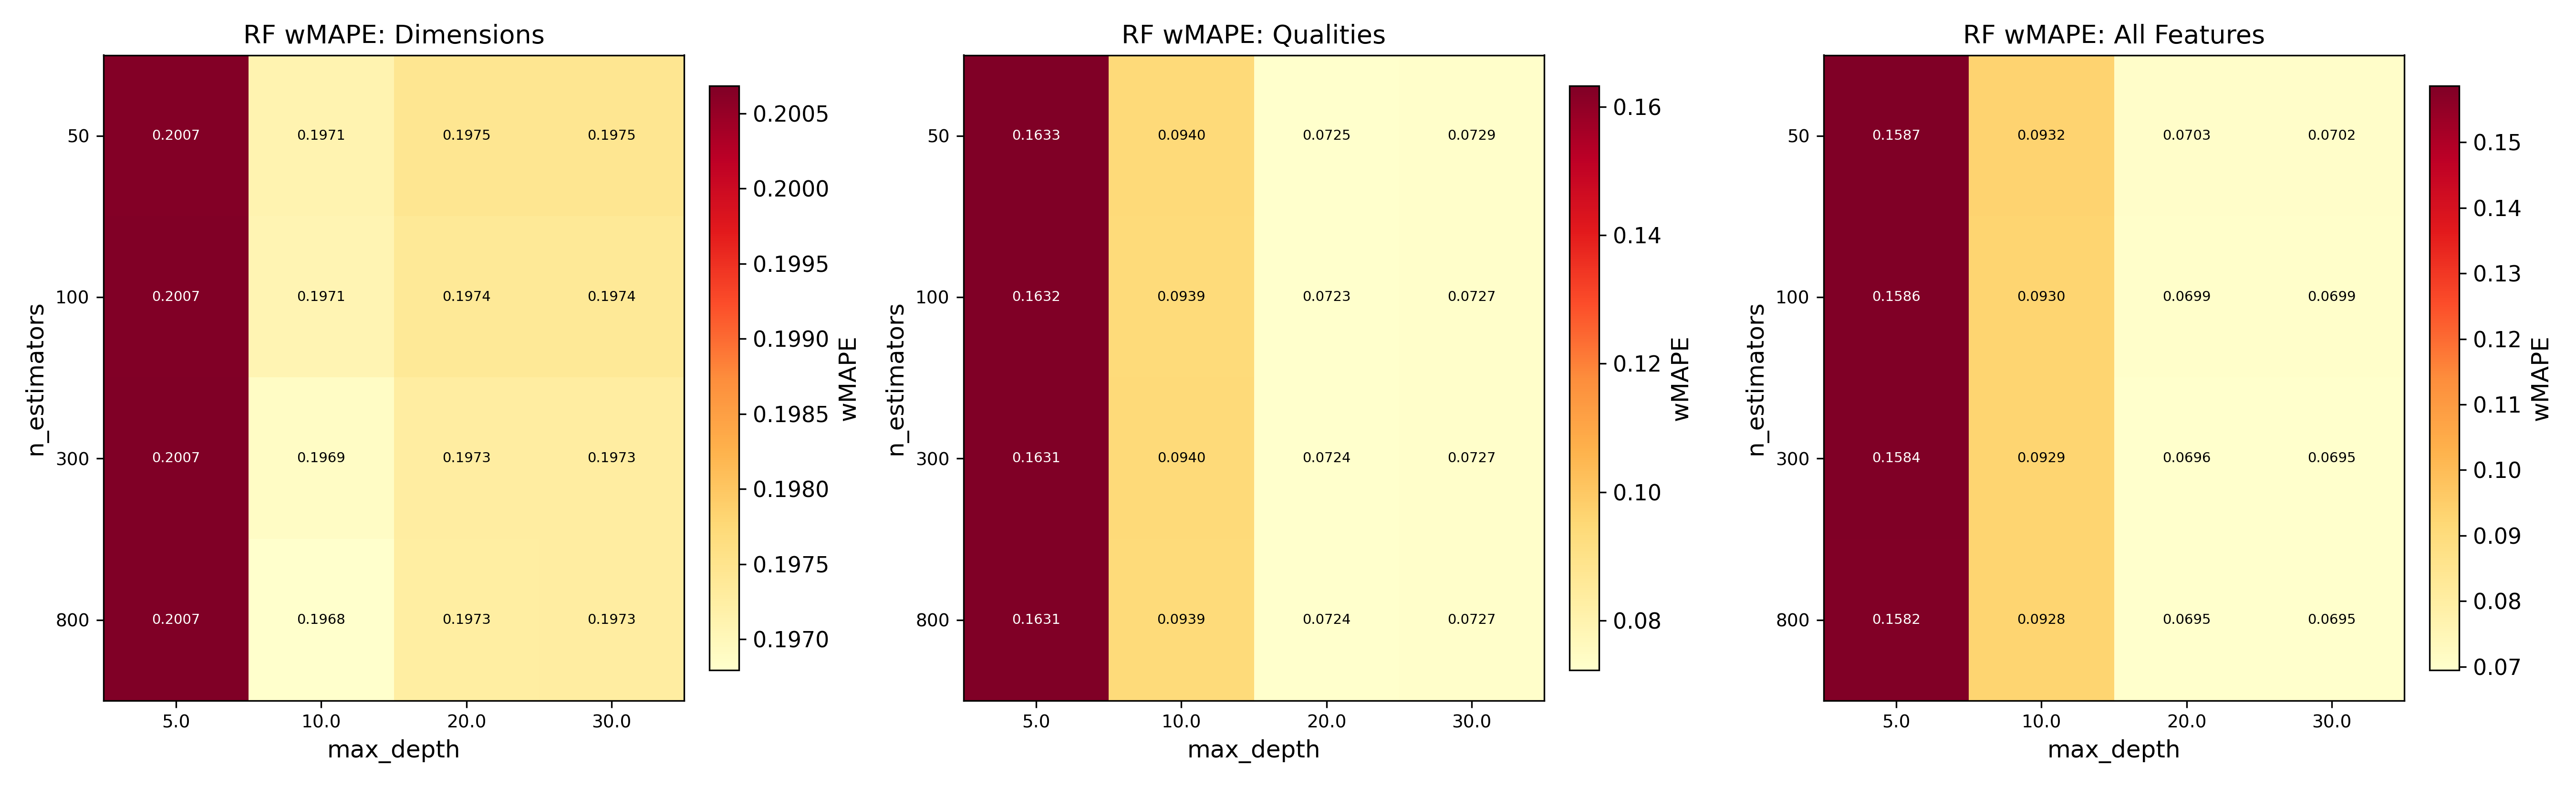
\includegraphics[width=\columnwidth]{plots/rf_heatmaps_all_sweeps.png}}
\caption{Random Forest wMAPE heatmaps (n\_estimators vs.\ max\_depth) for each feature set. Optimal max\_depth increases with feature complexity: 10 for dimensions, 20 for qualities, unlimited for all features.}
\label{fig:rf_heatmaps}
\end{figure}

\begin{itemize}
\item \textbf{max\_depth scales with feature complexity}: The dimensions sweep optimizes at depth 10, qualities at depth 20, and all-features at unlimited depth. More features require deeper trees to capture interactions.
\item \textbf{n\_estimators shows diminishing returns}: Performance gains taper rapidly beyond 100--300 trees. The marginal improvement from 300 to 800 trees is consistently $<0.001$ wMAPE.
\item \textbf{Shallow trees are catastrophic}: max\_depth$=5$ produces the worst results in all sweeps, especially for qualities (wMAPE $\approx 0.16$ vs.\ 0.07 at depth 20).
\end{itemize}

\subsubsection{n\_estimators vs.\ min\_samples\_leaf Interaction}

Fig.~\ref{fig:nest_by_leaf} isolates the interaction between \texttt{n\_estimators} and \texttt{min\_samples\_leaf} by plotting wMAPE curves at each leaf value (marginalised by taking the best max\_depth). For the qualities and all-features sweeps, the curves for leaf$=1$ and leaf$=2$ are nearly indistinguishable, while leaf$\ge 8$ imposes a consistent penalty. For the dimensions sweep, where the feature space is simple and the wMAPE range is narrow, leaf size has almost no effect.

\begin{figure}[htbp]
\centerline{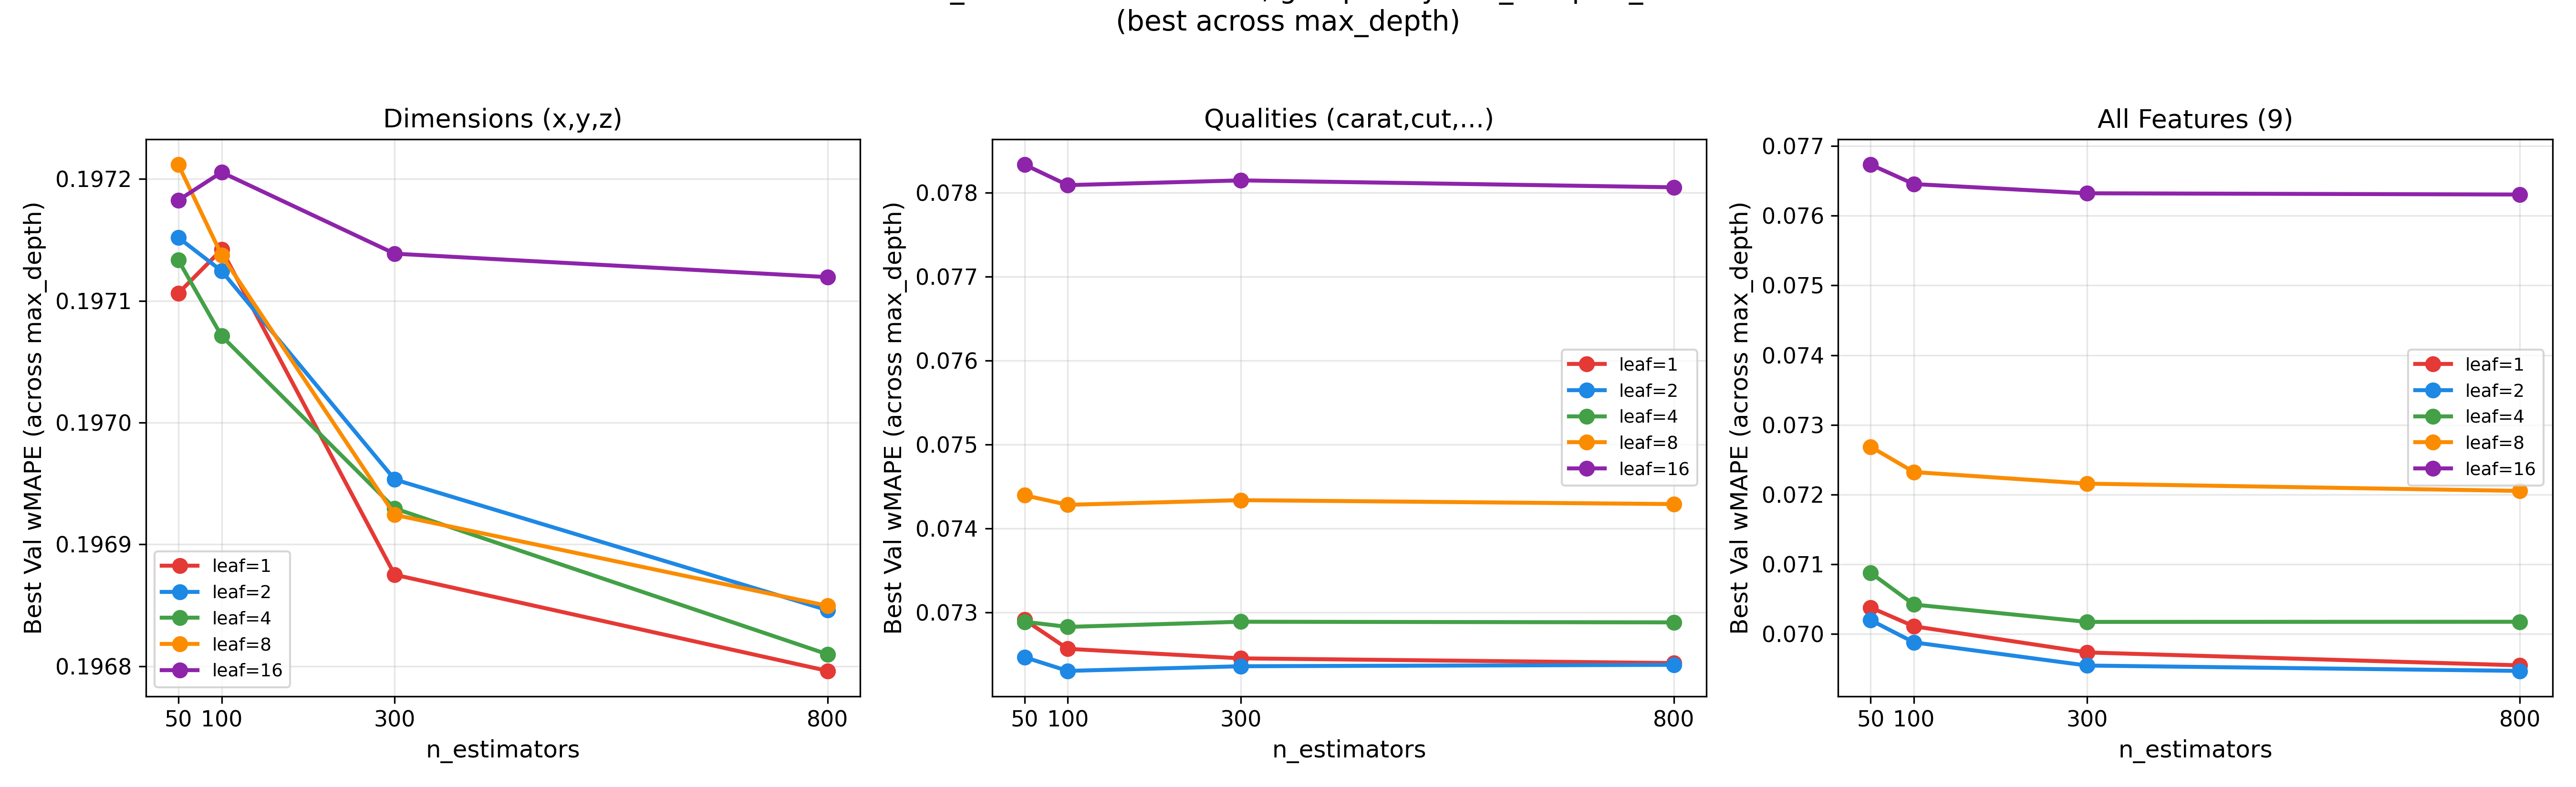
\includegraphics[width=\columnwidth]{plots/param_nestimators_by_leaf.png}}
\caption{RF: n\_estimators vs.\ best wMAPE, with one curve per min\_samples\_leaf value (best across all max\_depth). Larger leaf sizes penalize the richer feature sets more.}
\label{fig:nest_by_leaf}
\end{figure}

\subsubsection{max\_depth vs.\ min\_samples\_leaf Interaction}

Fig.~\ref{fig:depth_by_leaf} shows how \texttt{max\_depth} and \texttt{min\_samples\_leaf} jointly affect wMAPE. When depth is low (5--10), all leaf values perform similarly because the tree is already constrained. At higher depths ($\ge 20$ or unlimited), lower leaf values (1--2) clearly separate from higher values (8--16), indicating that deeper trees benefit from finer-grained leaf partitioning.

\begin{figure}[htbp]
\centerline{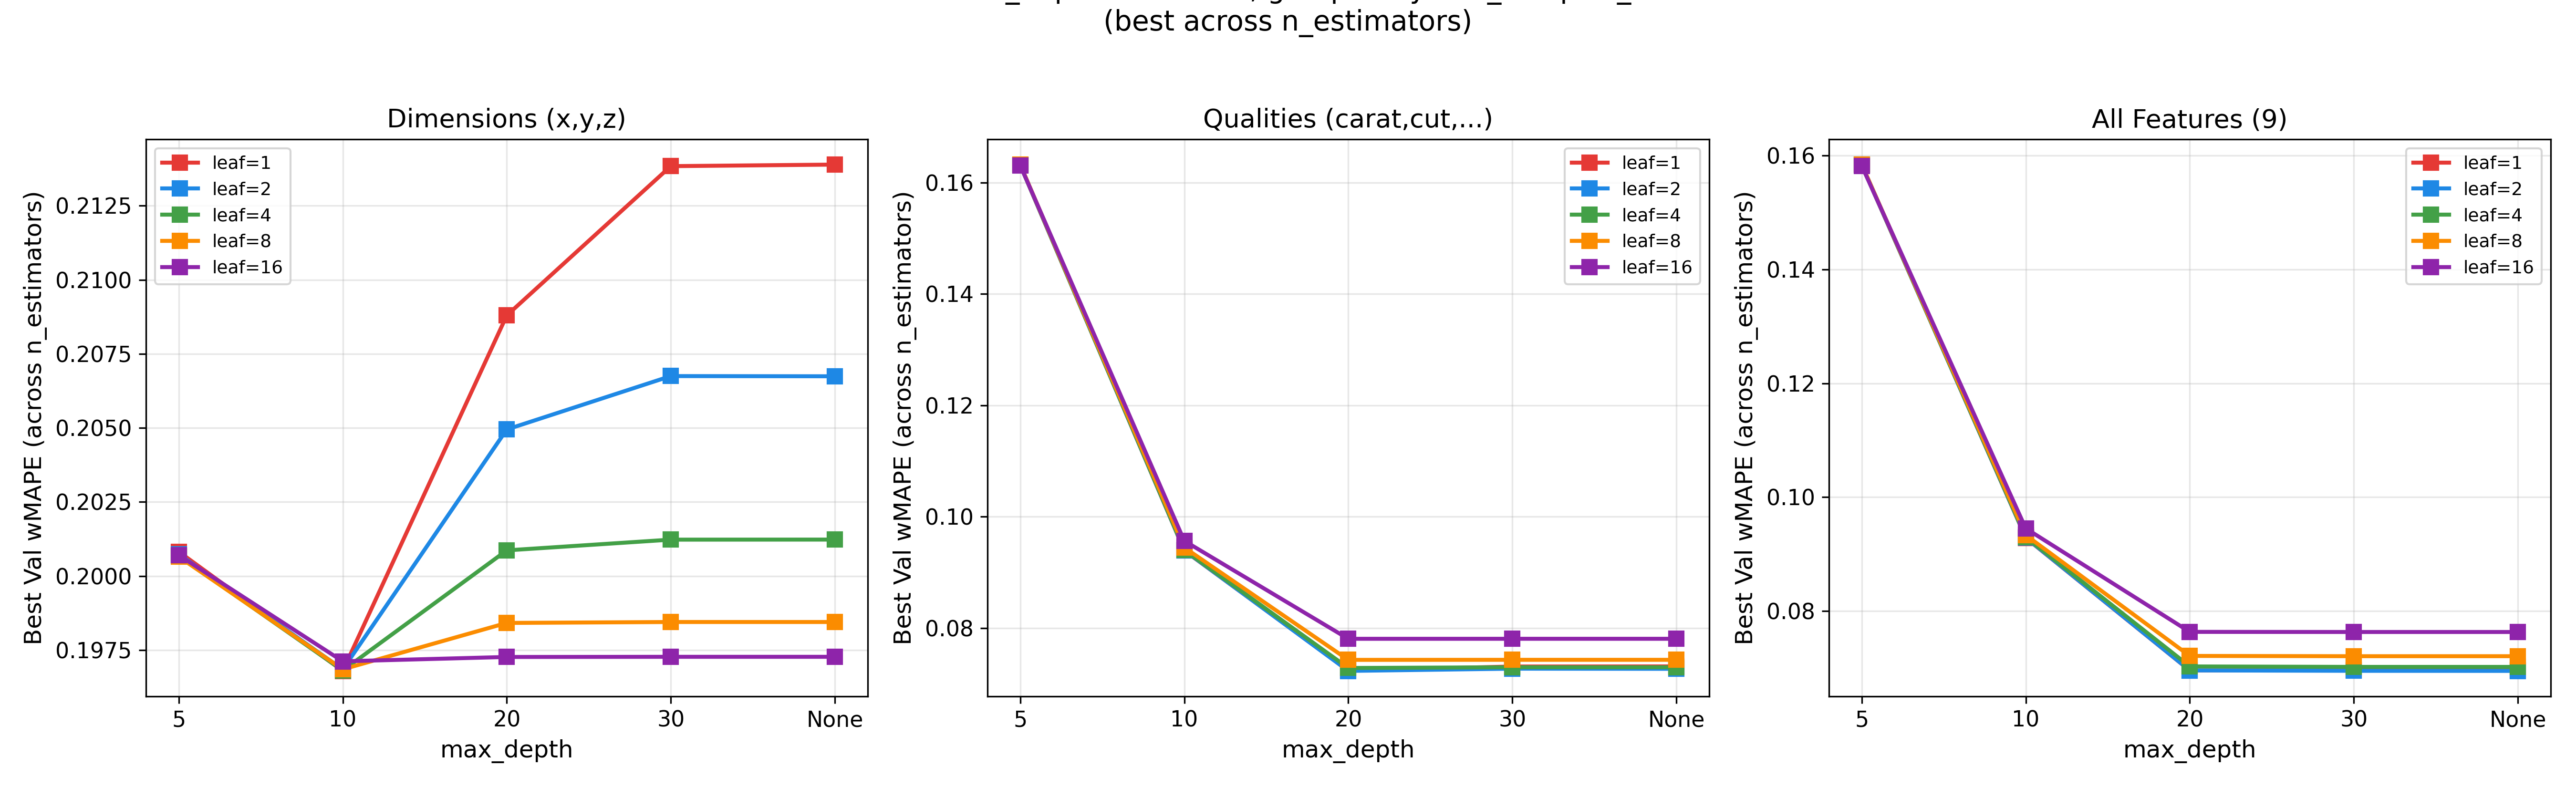
\includegraphics[width=\columnwidth]{plots/param_maxdepth_by_leaf.png}}
\caption{RF: max\_depth vs.\ best wMAPE, with one curve per min\_samples\_leaf (best across n\_estimators). At high depth, leaf=1--2 outperforms leaf$\ge$8.}
\label{fig:depth_by_leaf}
\end{figure}

Fig.~\ref{fig:leaf_depth_heat} provides a complementary heatmap view of this interaction. The bottom-left corner (low leaf, high depth) consistently produces the best wMAPE, while the top-left corner (high leaf, low depth) produces the worst.

\begin{figure}[htbp]
\centerline{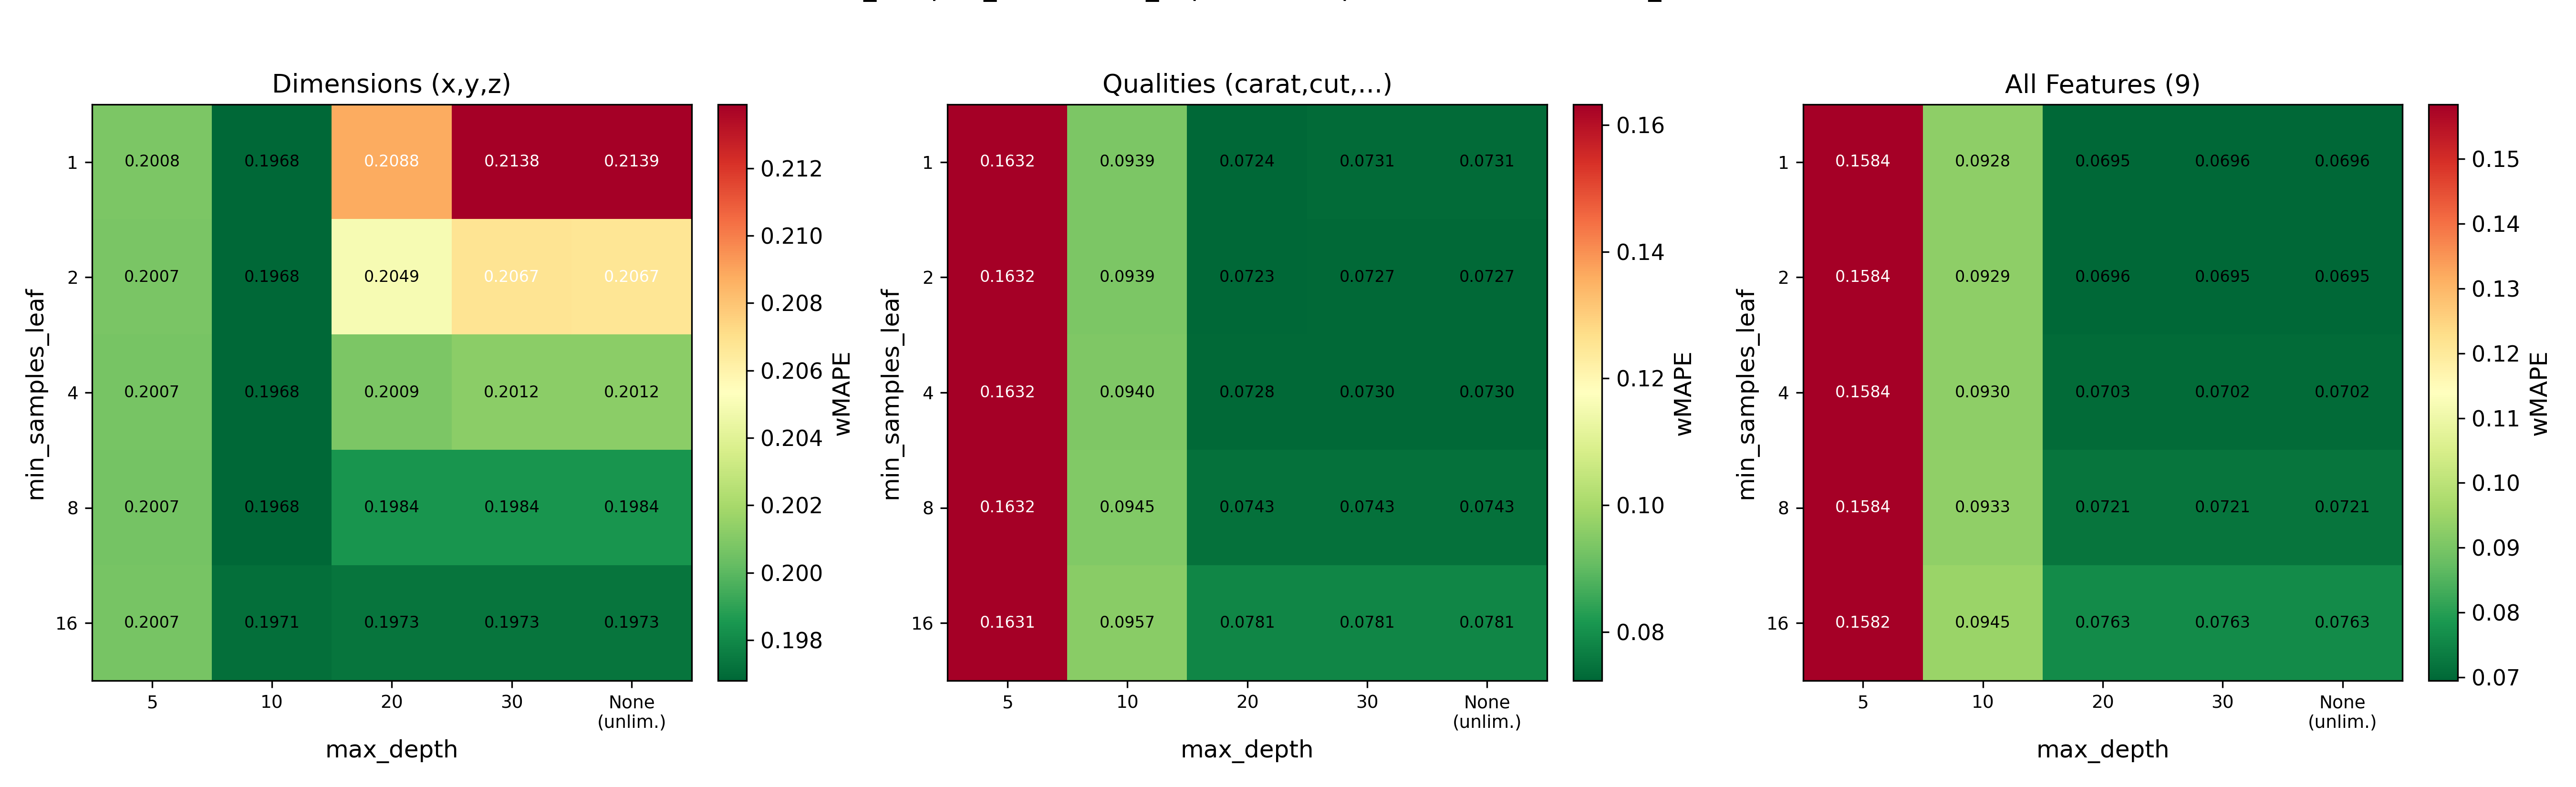
\includegraphics[width=\columnwidth]{plots/rf_leaf_vs_depth_heatmap.png}}
\caption{RF heatmap: min\_samples\_leaf vs.\ max\_depth (best wMAPE across n\_estimators). Best region is low leaf with high depth.}
\label{fig:leaf_depth_heat}
\end{figure}

\subsubsection{n\_estimators vs.\ max\_depth Interaction}

Fig.~\ref{fig:nest_by_depth} directly compares how the number of trees interacts with tree depth. At depth$=5$, adding trees beyond 50 provides no meaningful improvement (the trees are individually too weak). At depth$\ge 20$, more trees consistently reduce variance and improve wMAPE, though returns diminish beyond 300.

\begin{figure}[htbp]
\centerline{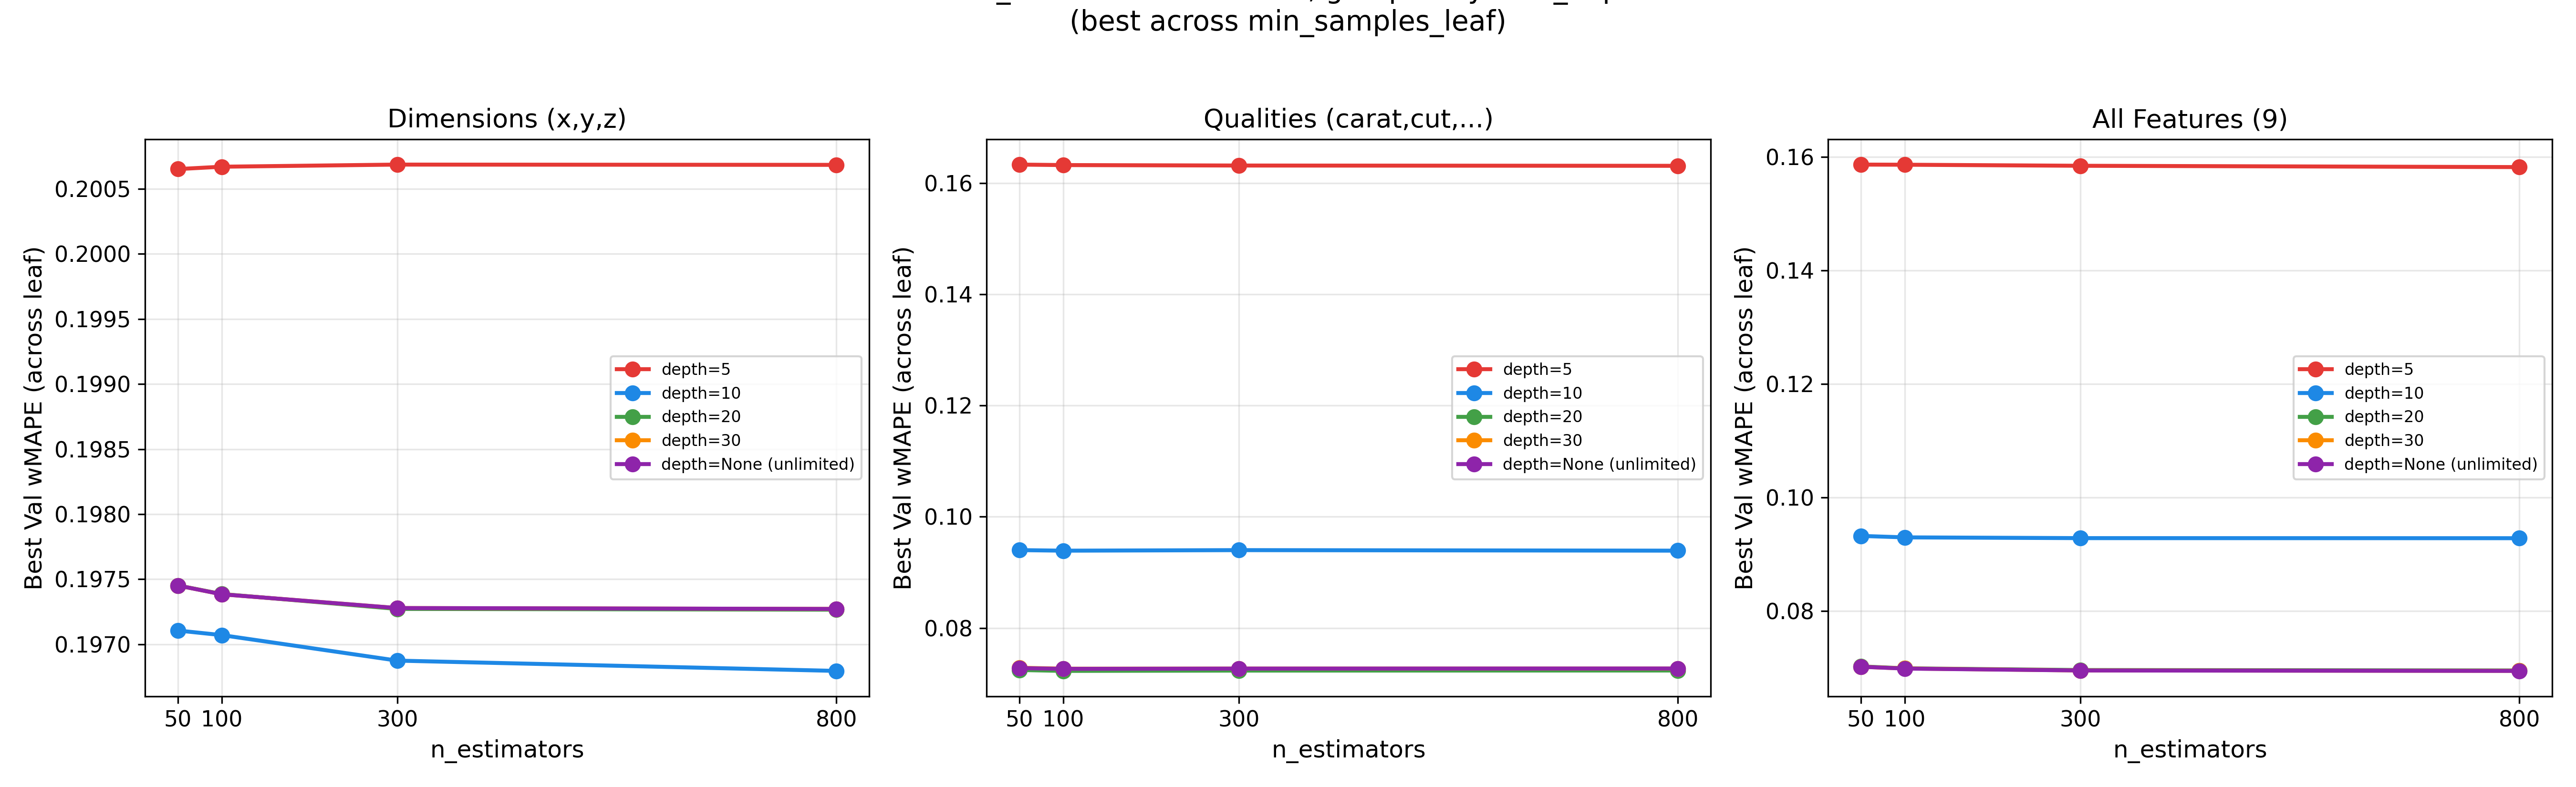
\includegraphics[width=\columnwidth]{plots/param_nestimators_by_depth.png}}
\caption{RF: n\_estimators vs.\ best wMAPE, with one curve per max\_depth (best across min\_samples\_leaf). More trees help most when individual trees are deep.}
\label{fig:nest_by_depth}
\end{figure}

\subsubsection{Three-Way Interaction (All Features)}

Fig.~\ref{fig:3way} provides the most detailed view of RF behavior by showing \texttt{n\_estimators} $\times$ \texttt{min\_samples\_leaf} heatmaps for every \texttt{max\_depth} value in the all-features sweep. At depth$=5$, the entire heatmap is nearly uniform (all combos are poor); at depth$\ge 20$, the best results cluster in the low-leaf, high-estimator corner.

\begin{figure}[htbp]
\centerline{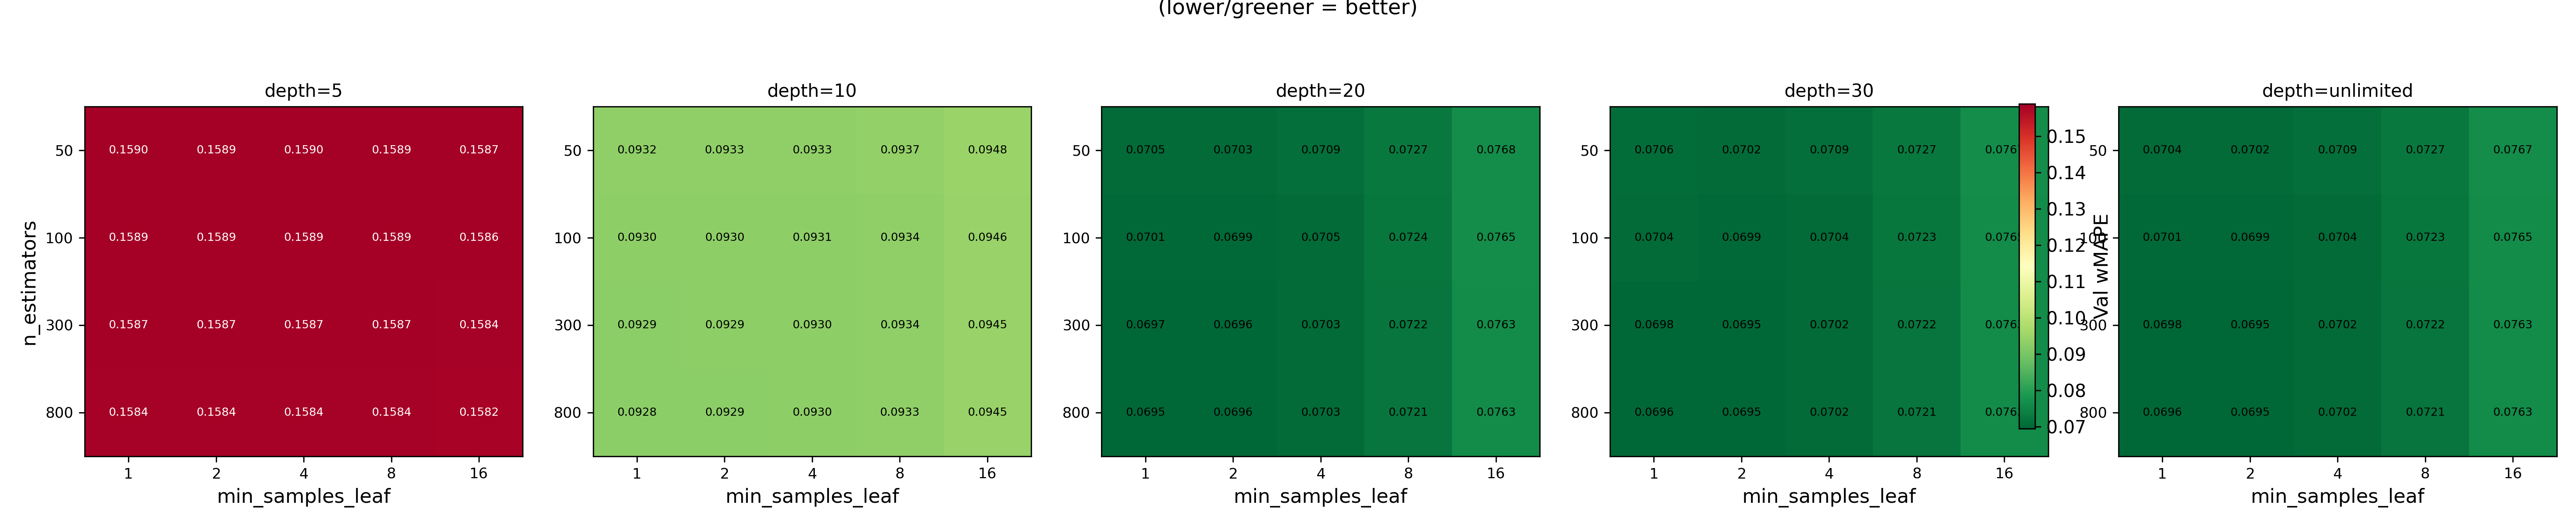
\includegraphics[width=\columnwidth]{plots/rf_3way_heatmap_allfeatures.png}}
\caption{RF three-way interaction in the all-features sweep: n\_estimators $\times$ min\_samples\_leaf heatmaps for each max\_depth. Performance improves left-to-right (increasing depth) and bottom-to-top (more trees, lower leaf).}
\label{fig:3way}
\end{figure}

\subsubsection{All-Combo Scatter and Top vs.\ Bottom Configurations}

Fig.~\ref{fig:scatter} plots every individual RF configuration with n\_estimators on the x-axis and wMAPE on the y-axis, color-coded by min\_samples\_leaf and sized by max\_depth. The scatter confirms that the best configurations (lowest wMAPE) are consistently blue/red (leaf$=1$--$2$) with large markers (high depth), positioned at higher n\_estimators.

\begin{figure}[htbp]
\centerline{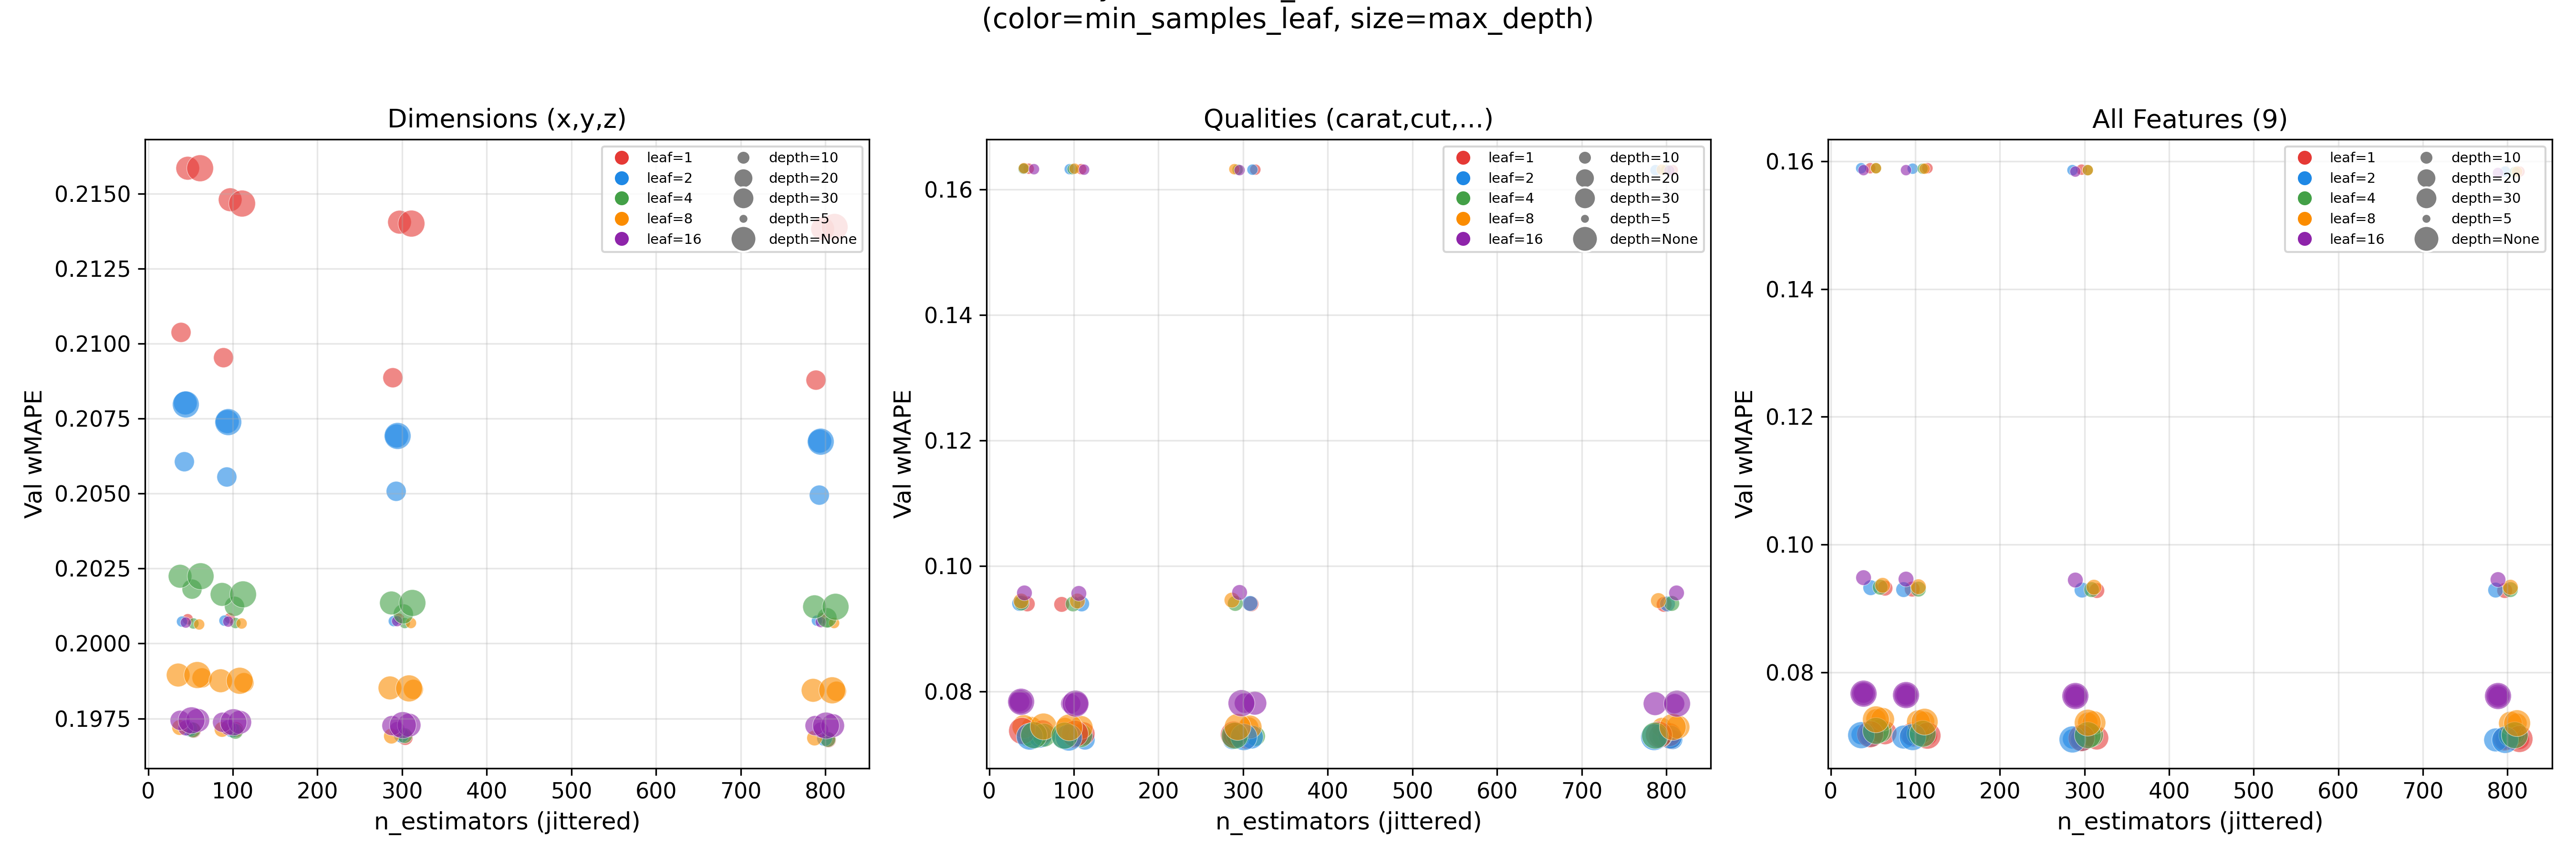
\includegraphics[width=\columnwidth]{plots/rf_scatter_all_combos.png}}
\caption{RF: every configuration plotted. Color encodes min\_samples\_leaf, marker size encodes max\_depth. Best combos cluster at high n\_estimators, low leaf, high depth.}
\label{fig:scatter}
\end{figure}

Fig.~\ref{fig:topbot} directly compares the parameter distributions of the top-10 vs.\ bottom-10 configurations (by wMAPE) in the all-features sweep. The top-10 overwhelmingly use \texttt{n\_estimators}$\ge 300$, \texttt{min\_samples\_leaf}$\le 2$, and \texttt{max\_depth}$\ge 20$ or unlimited. The bottom-10 cluster at \texttt{max\_depth}$=5$.

\begin{figure}[htbp]
\centerline{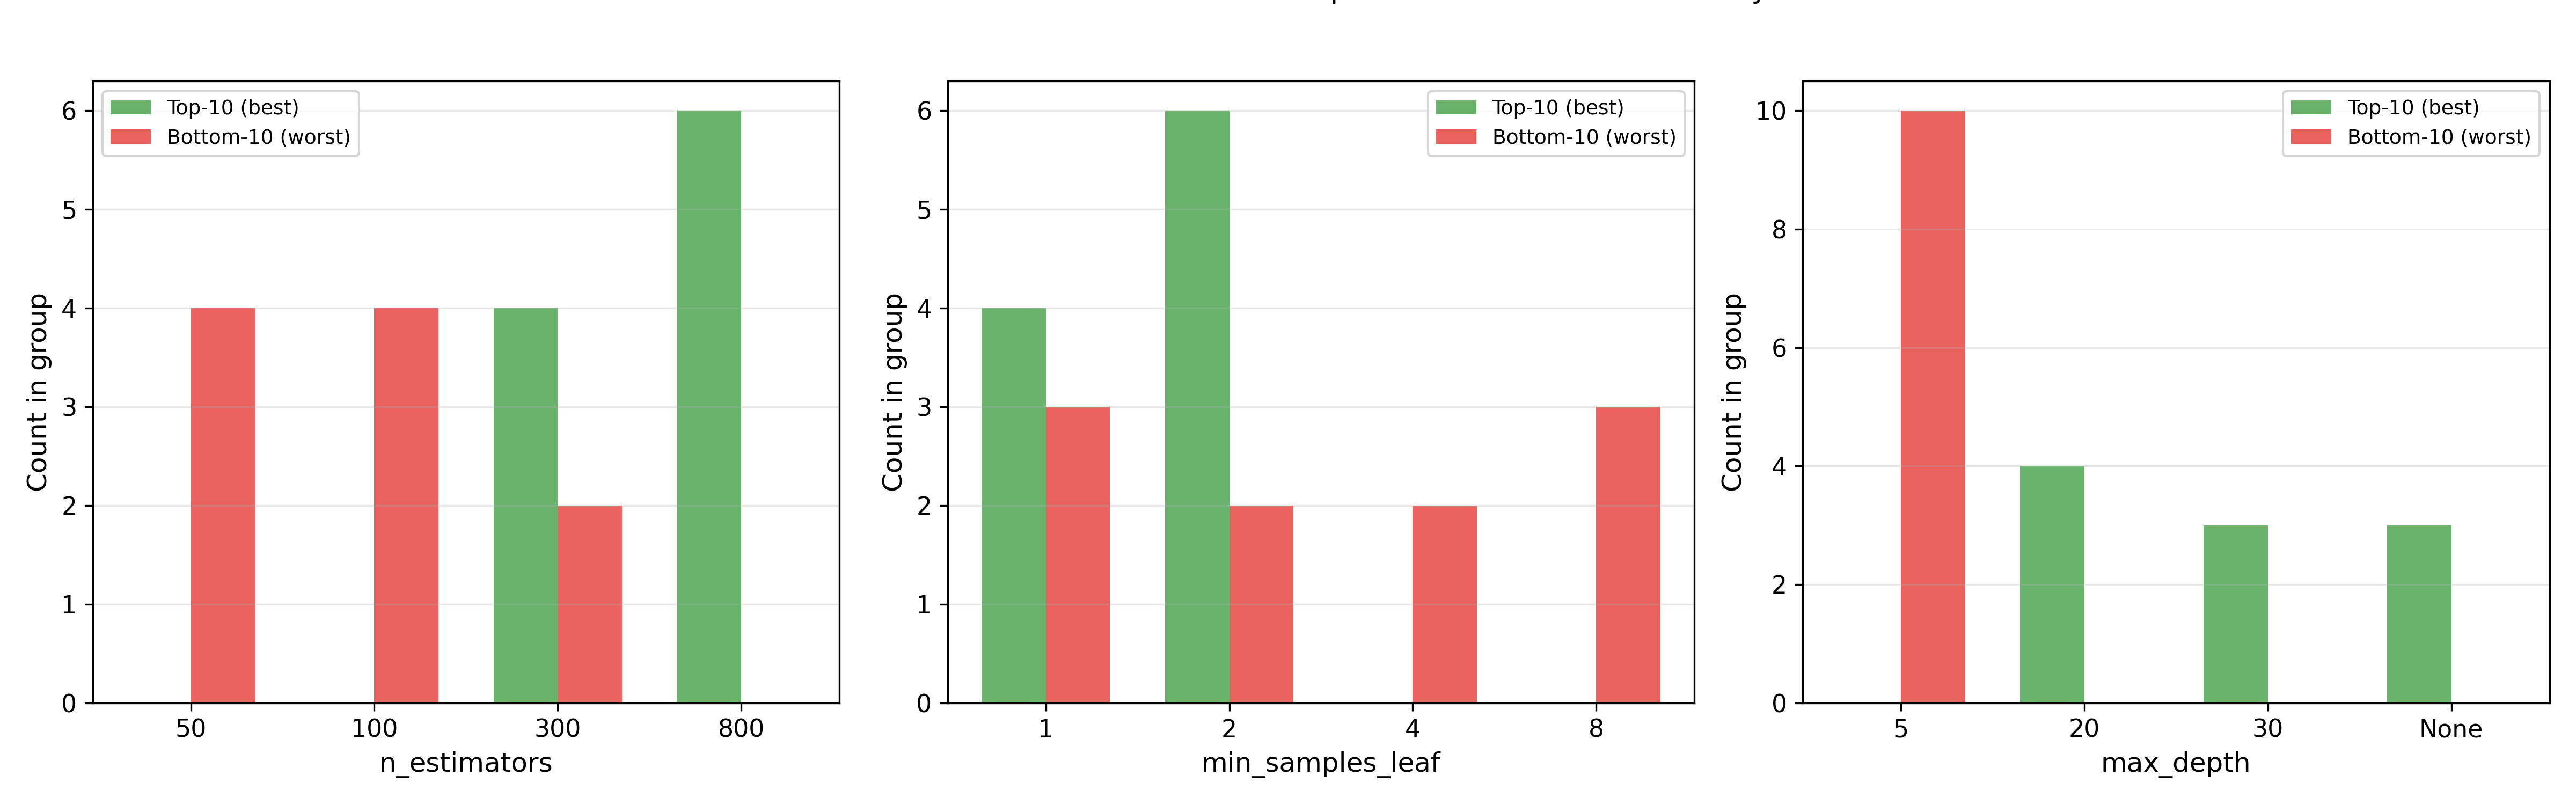
\includegraphics[width=\columnwidth]{plots/rf_top_vs_bottom_params.png}}
\caption{RF All Features: parameter frequency in the 10 best (green) vs.\ 10 worst (red) configurations. Best combos use $\ge$300 trees, leaf$\le$2, and depth$\ge$20.}
\label{fig:topbot}
\end{figure}

\subsection{Marginal Parameter Sensitivity (All Models)}

Fig.~\ref{fig:marginal} presents a unified view of all six hyperparameters across all three model types. For each parameter value, both the mean wMAPE (averaged over all other params) and the best wMAPE (minimum over all other params) are plotted across all three sweeps. This reveals:

\begin{figure}[htbp]
\centerline{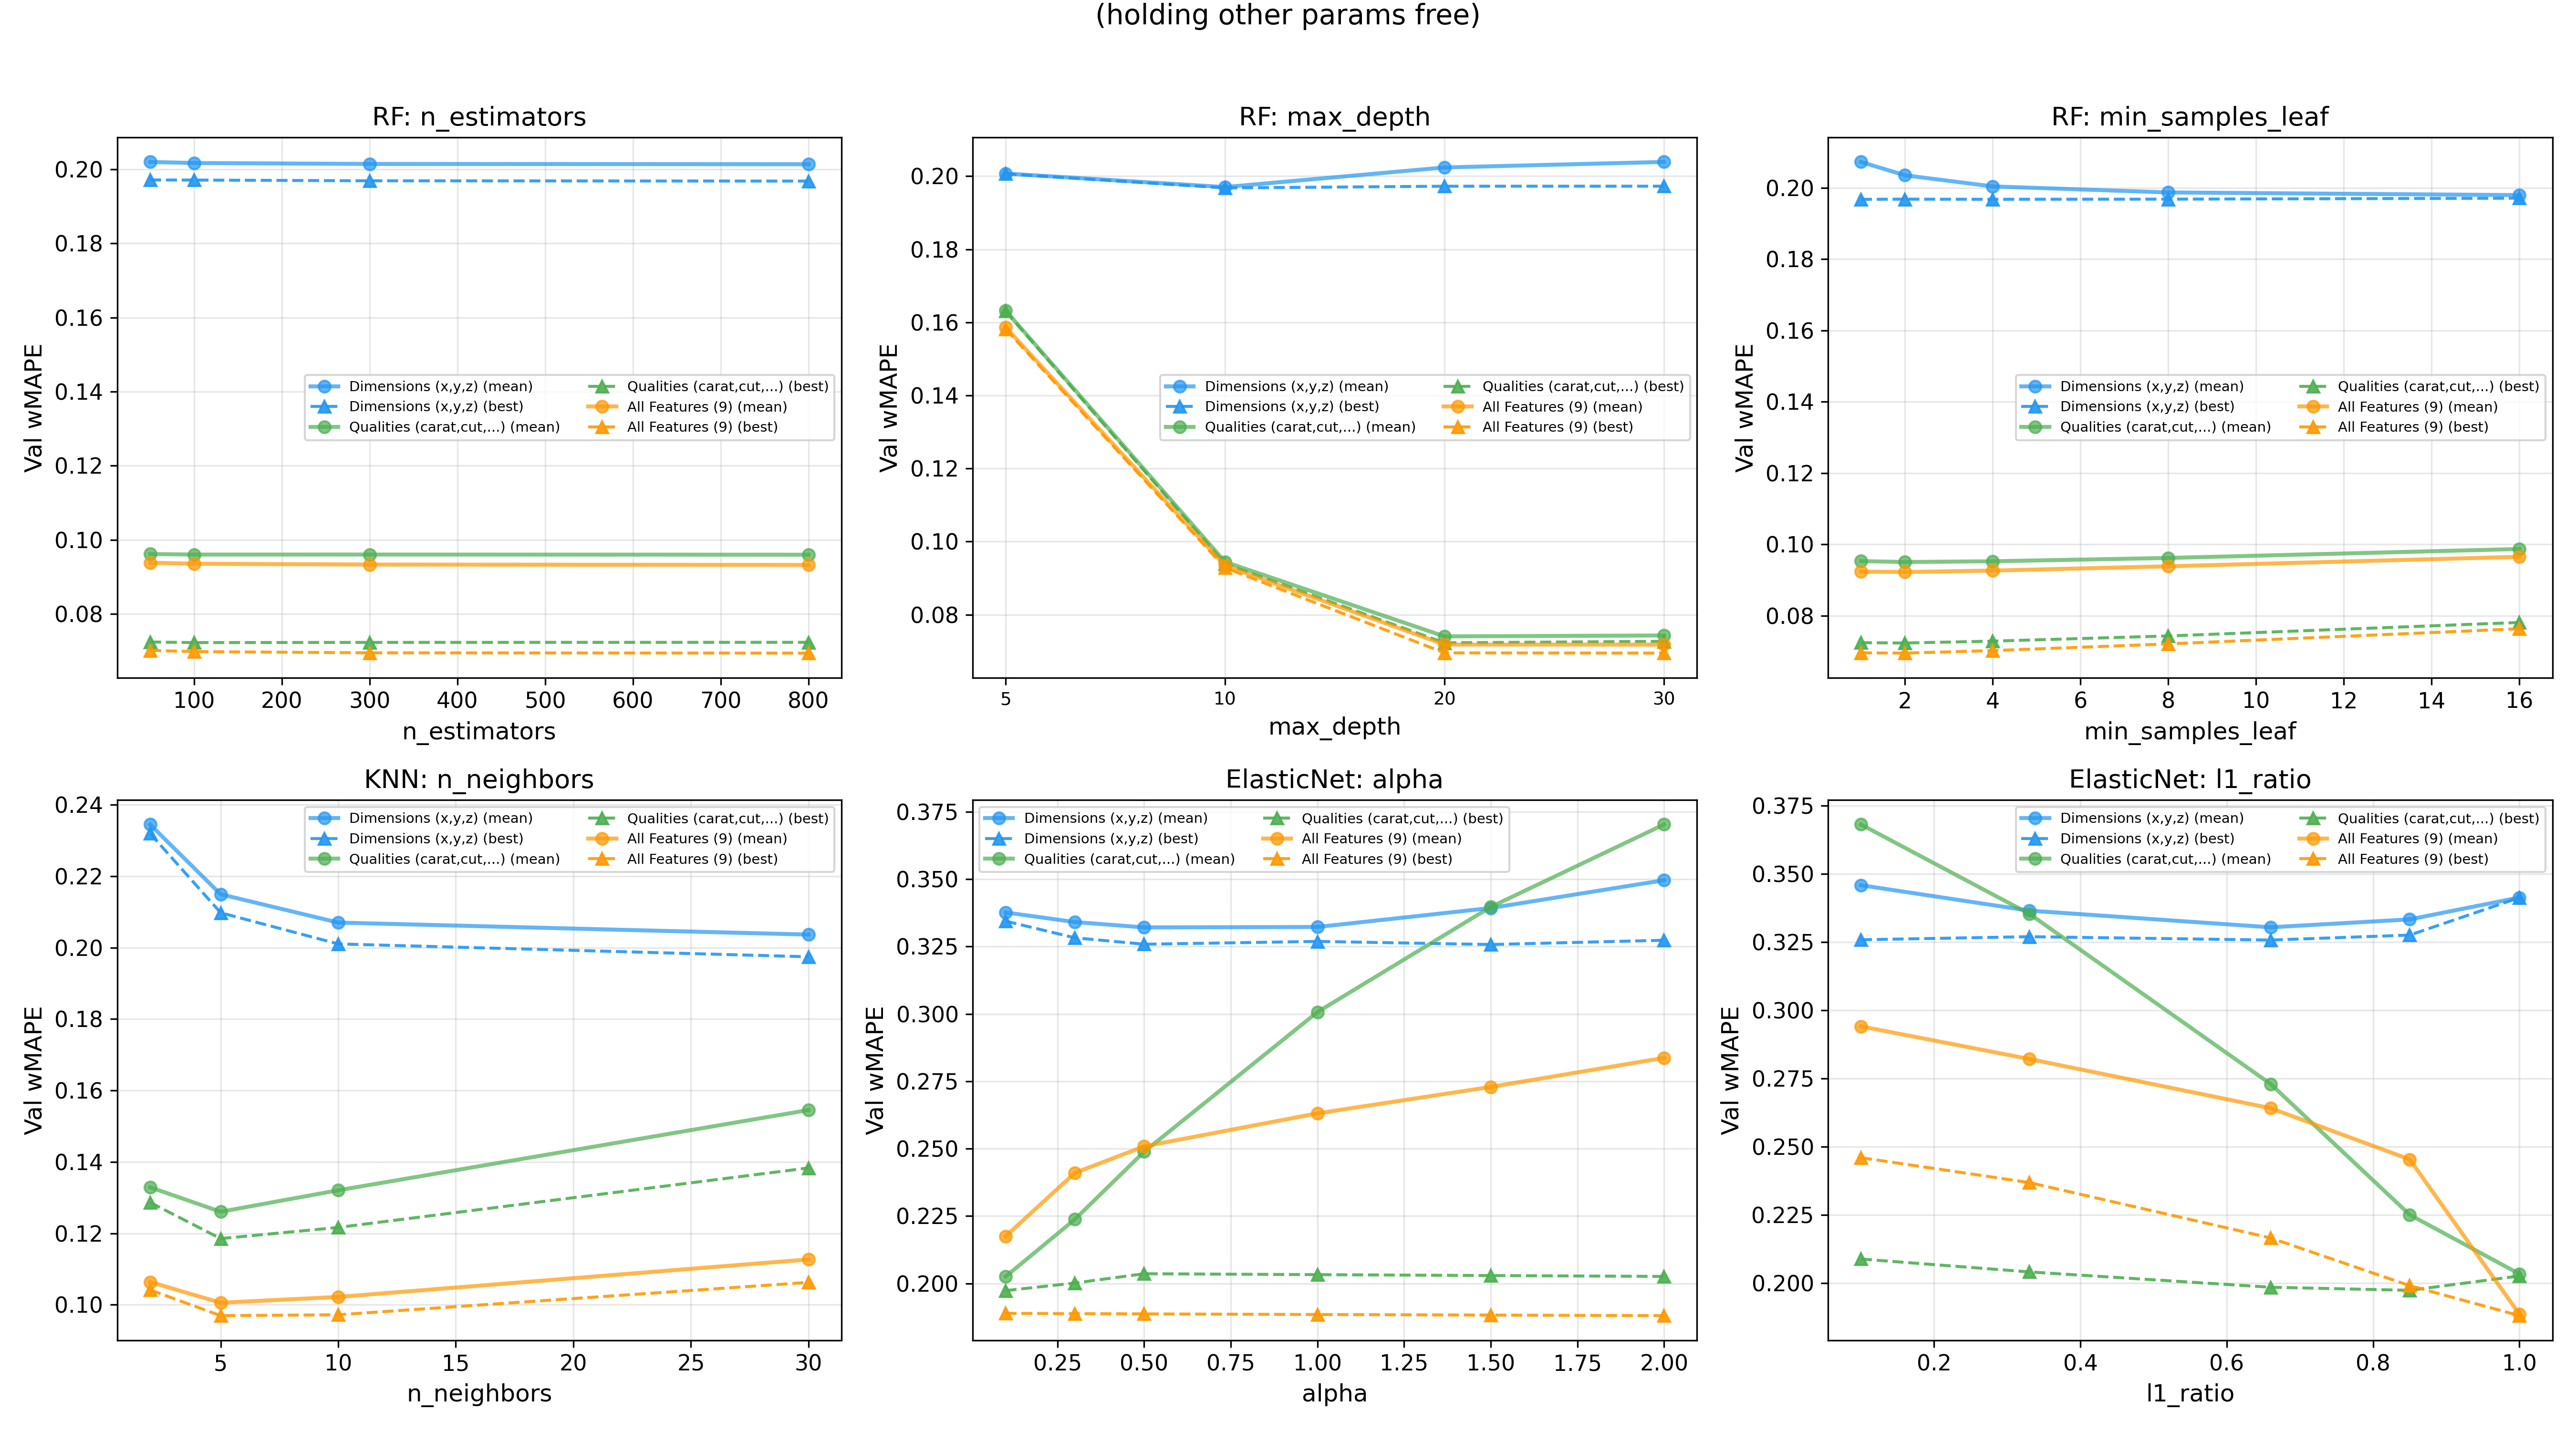
\includegraphics[width=\columnwidth]{plots/param_marginal_sensitivity.png}}
\caption{Marginal sensitivity for all six hyperparameters. Solid lines show mean wMAPE; dashed lines show best wMAPE. RF parameters (top row) and KNN/ElasticNet parameters (bottom row) across all three sweeps.}
\label{fig:marginal}
\end{figure}

\begin{itemize}
\item \textbf{RF n\_estimators}: Mean and best curves diverge at low values (50 trees has high variance) but converge at 300+, confirming that $\ge 300$ trees are a safe default.
\item \textbf{RF max\_depth}: The steepest drop occurs from depth$=5$ to depth$=10$; beyond 20, marginal gains are minimal. For a heuristic, depth$=20$ is a good starting point.
\item \textbf{RF min\_samples\_leaf}: Mean wMAPE increases almost linearly with leaf size. Leaf$=1$--$2$ are the clear choice.
\item \textbf{KNN n\_neighbors}: Sweep-dependent; no single optimal $k$ exists. Start with $k=5$ for high-dimensional data.
\item \textbf{ElasticNet alpha}: Lower is better across all sweeps; alpha$=0.1$--$0.3$ is the safe range.
\item \textbf{ElasticNet l1\_ratio}: Mid-range values (0.33--0.66) balance L1 sparsity with L2 stability.
\end{itemize}

\subsection{KNN Hyperparameter Analysis}

Fig.~\ref{fig:knn} shows the effect of \texttt{n\_neighbors} on KNN performance. The optimal $k$ varies with feature dimensionality: $k=30$ for the 3-feature dimensions sweep (smooth feature space benefits from averaging), but $k=5$ for the 9-feature all-features sweep (curse of dimensionality makes distant neighbors less informative). Distance weighting consistently outperforms uniform weighting for the richer feature sets.

\begin{figure}[htbp]
\centerline{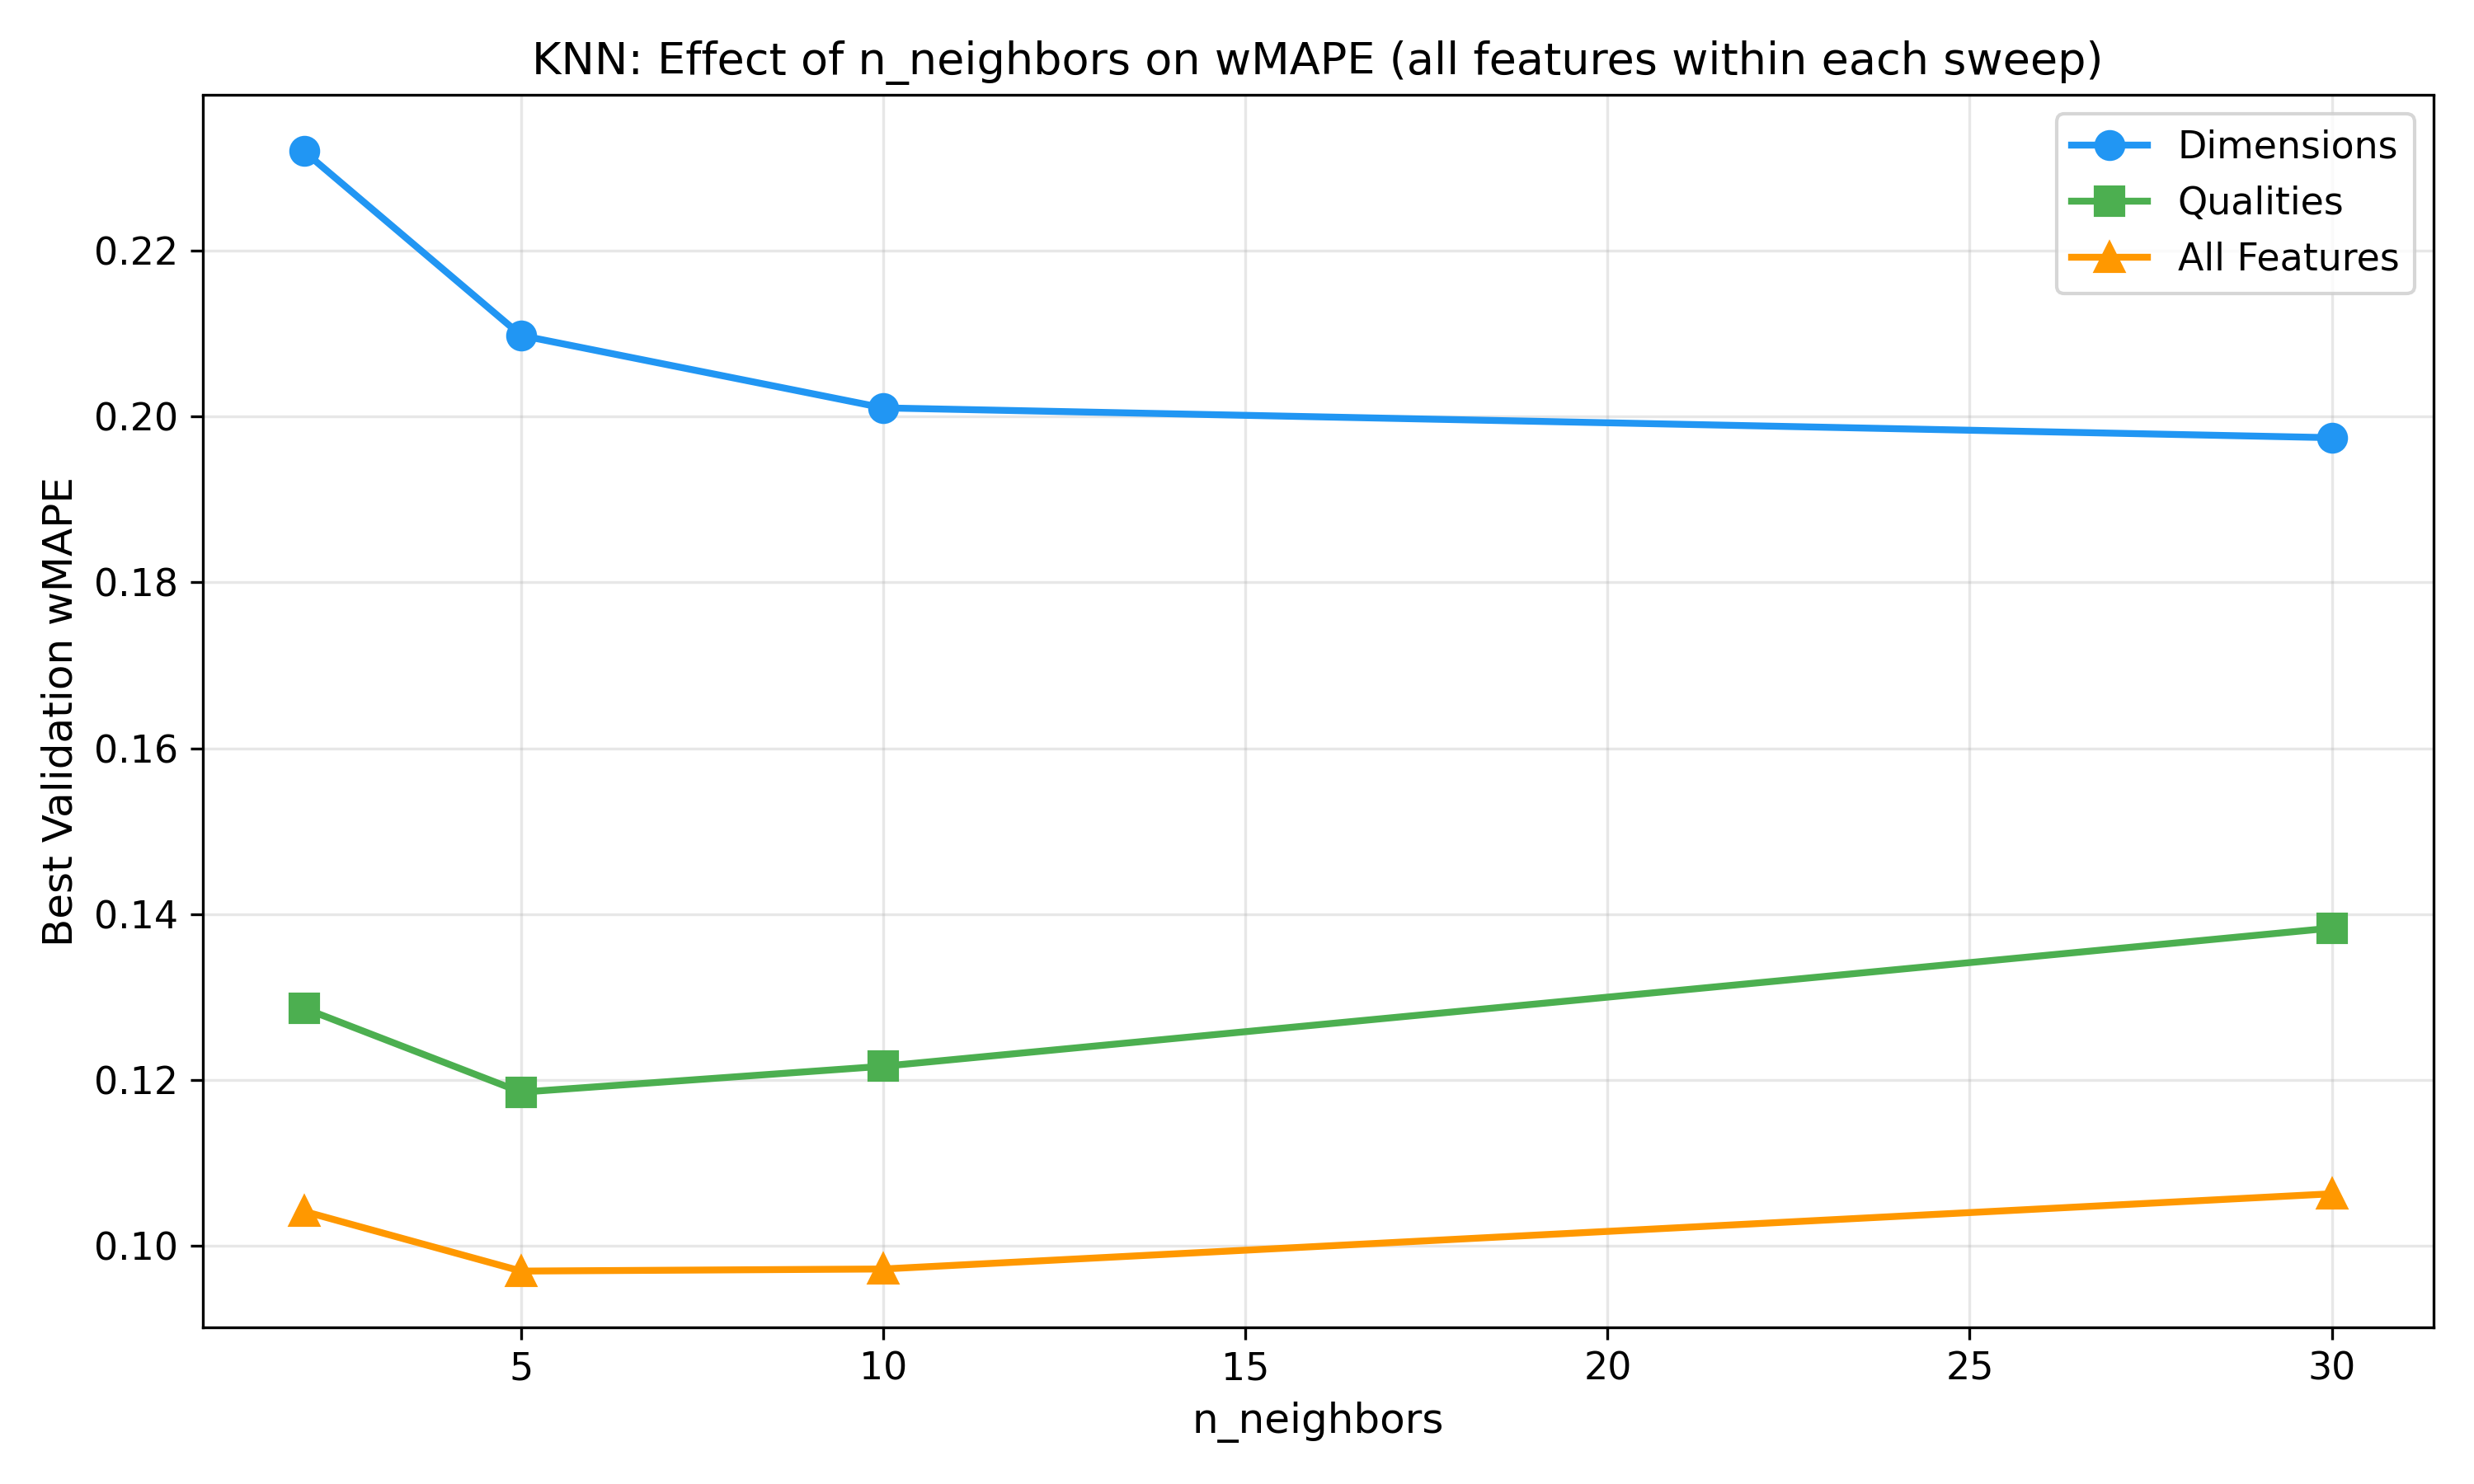
\includegraphics[width=\columnwidth]{plots/knn_neighbors_vs_wmape.png}}
\caption{KNN: validation wMAPE vs.\ n\_neighbors for each feature set. Optimal $k$ decreases as dimensionality increases.}
\label{fig:knn}
\end{figure}

\subsection{ElasticNet Hyperparameter Analysis}

Fig.~\ref{fig:elasticnet} shows ElasticNet performance across alpha and l1\_ratio values. Lower regularization strength (alpha$=0.1$--$0.3$) is preferred across all sweeps. Pure Lasso (l1\_ratio$=1.0$) zeros out useful features and performs worst, while balanced mixtures (l1\_ratio$=0.33$--$0.66$) provide the best linear model results.

\begin{figure}[htbp]
\centerline{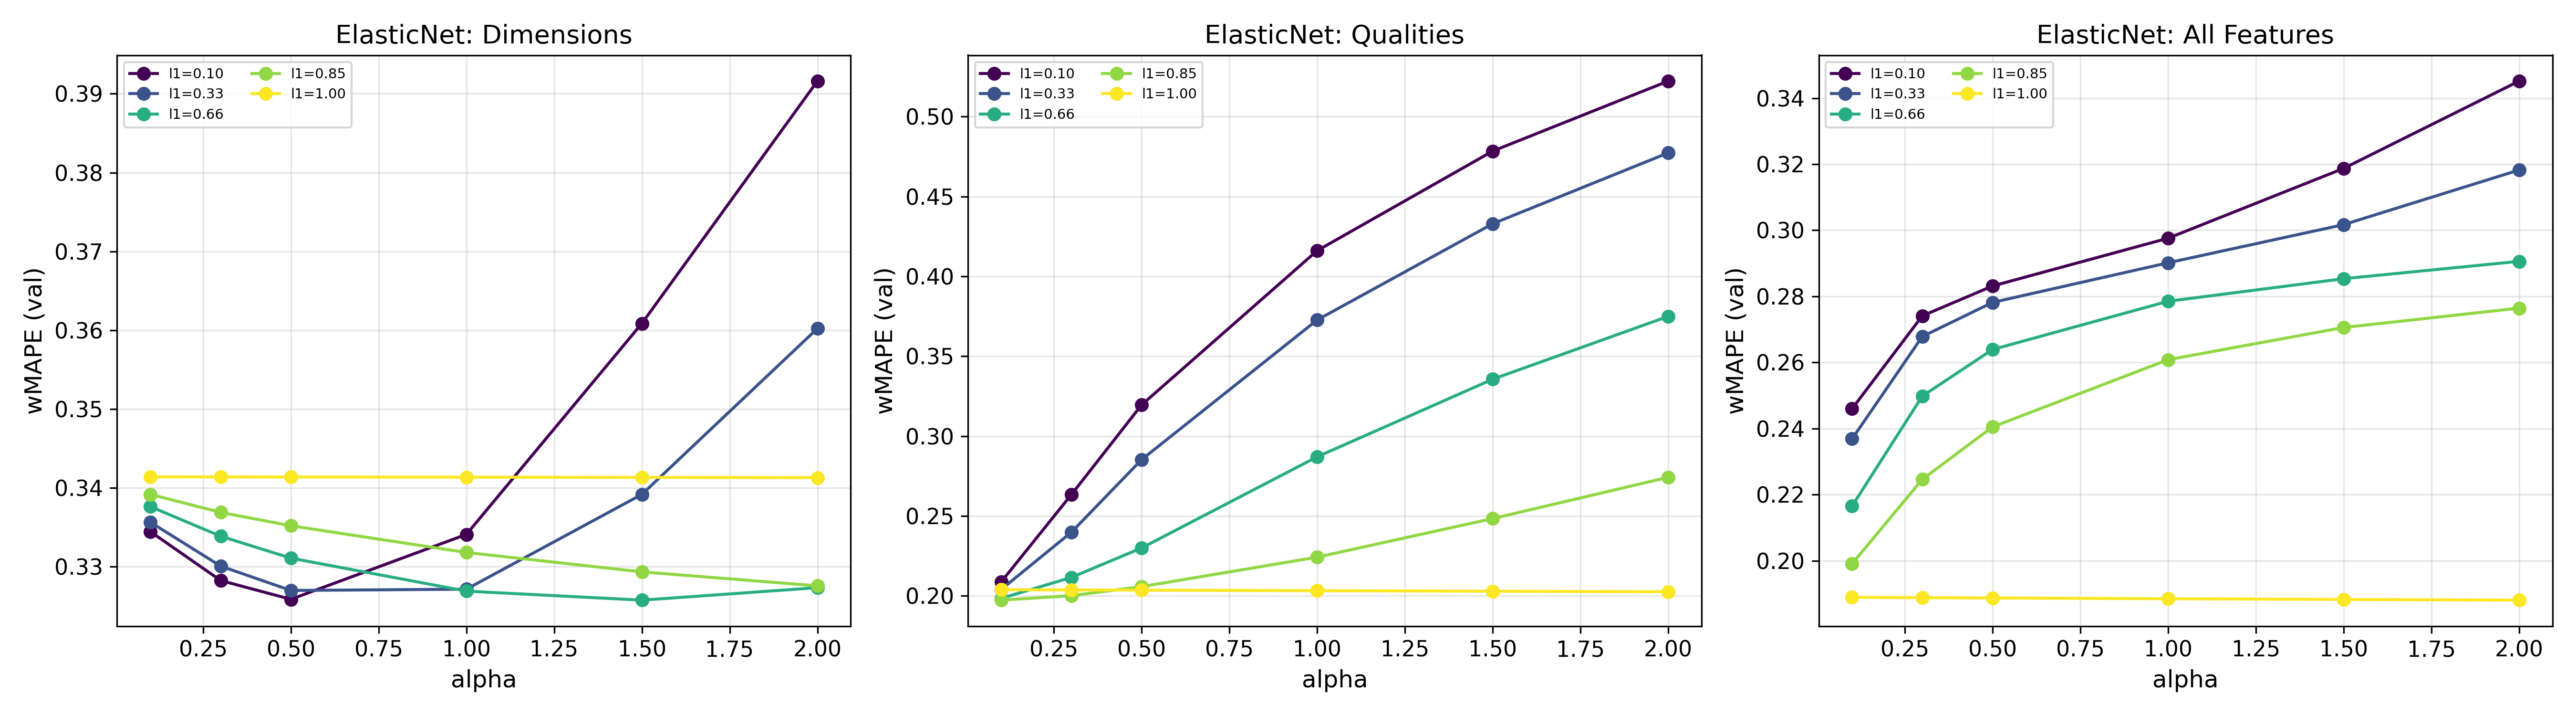
\includegraphics[width=\columnwidth]{plots/elasticnet_alpha_sweep.png}}
\caption{ElasticNet: validation wMAPE vs.\ alpha for different l1\_ratio values. Lower regularization and balanced L1/L2 mixing yield the best results.}
\label{fig:elasticnet}
\end{figure}

\subsection{Feature Importance}

\subsubsection{Gini Importance}

Fig.~\ref{fig:feature_imp} compares the top-10 Random Forest Gini importances between the qualities and all-features sweeps. In the qualities-only model, \texttt{carat} dominates at 88.4\%. When dimensions are added, importance splits between \texttt{carat} (48.9\%) and \texttt{y} (39.9\%), reflecting the strong collinearity between weight and physical width.

\begin{figure}[htbp]
\centerline{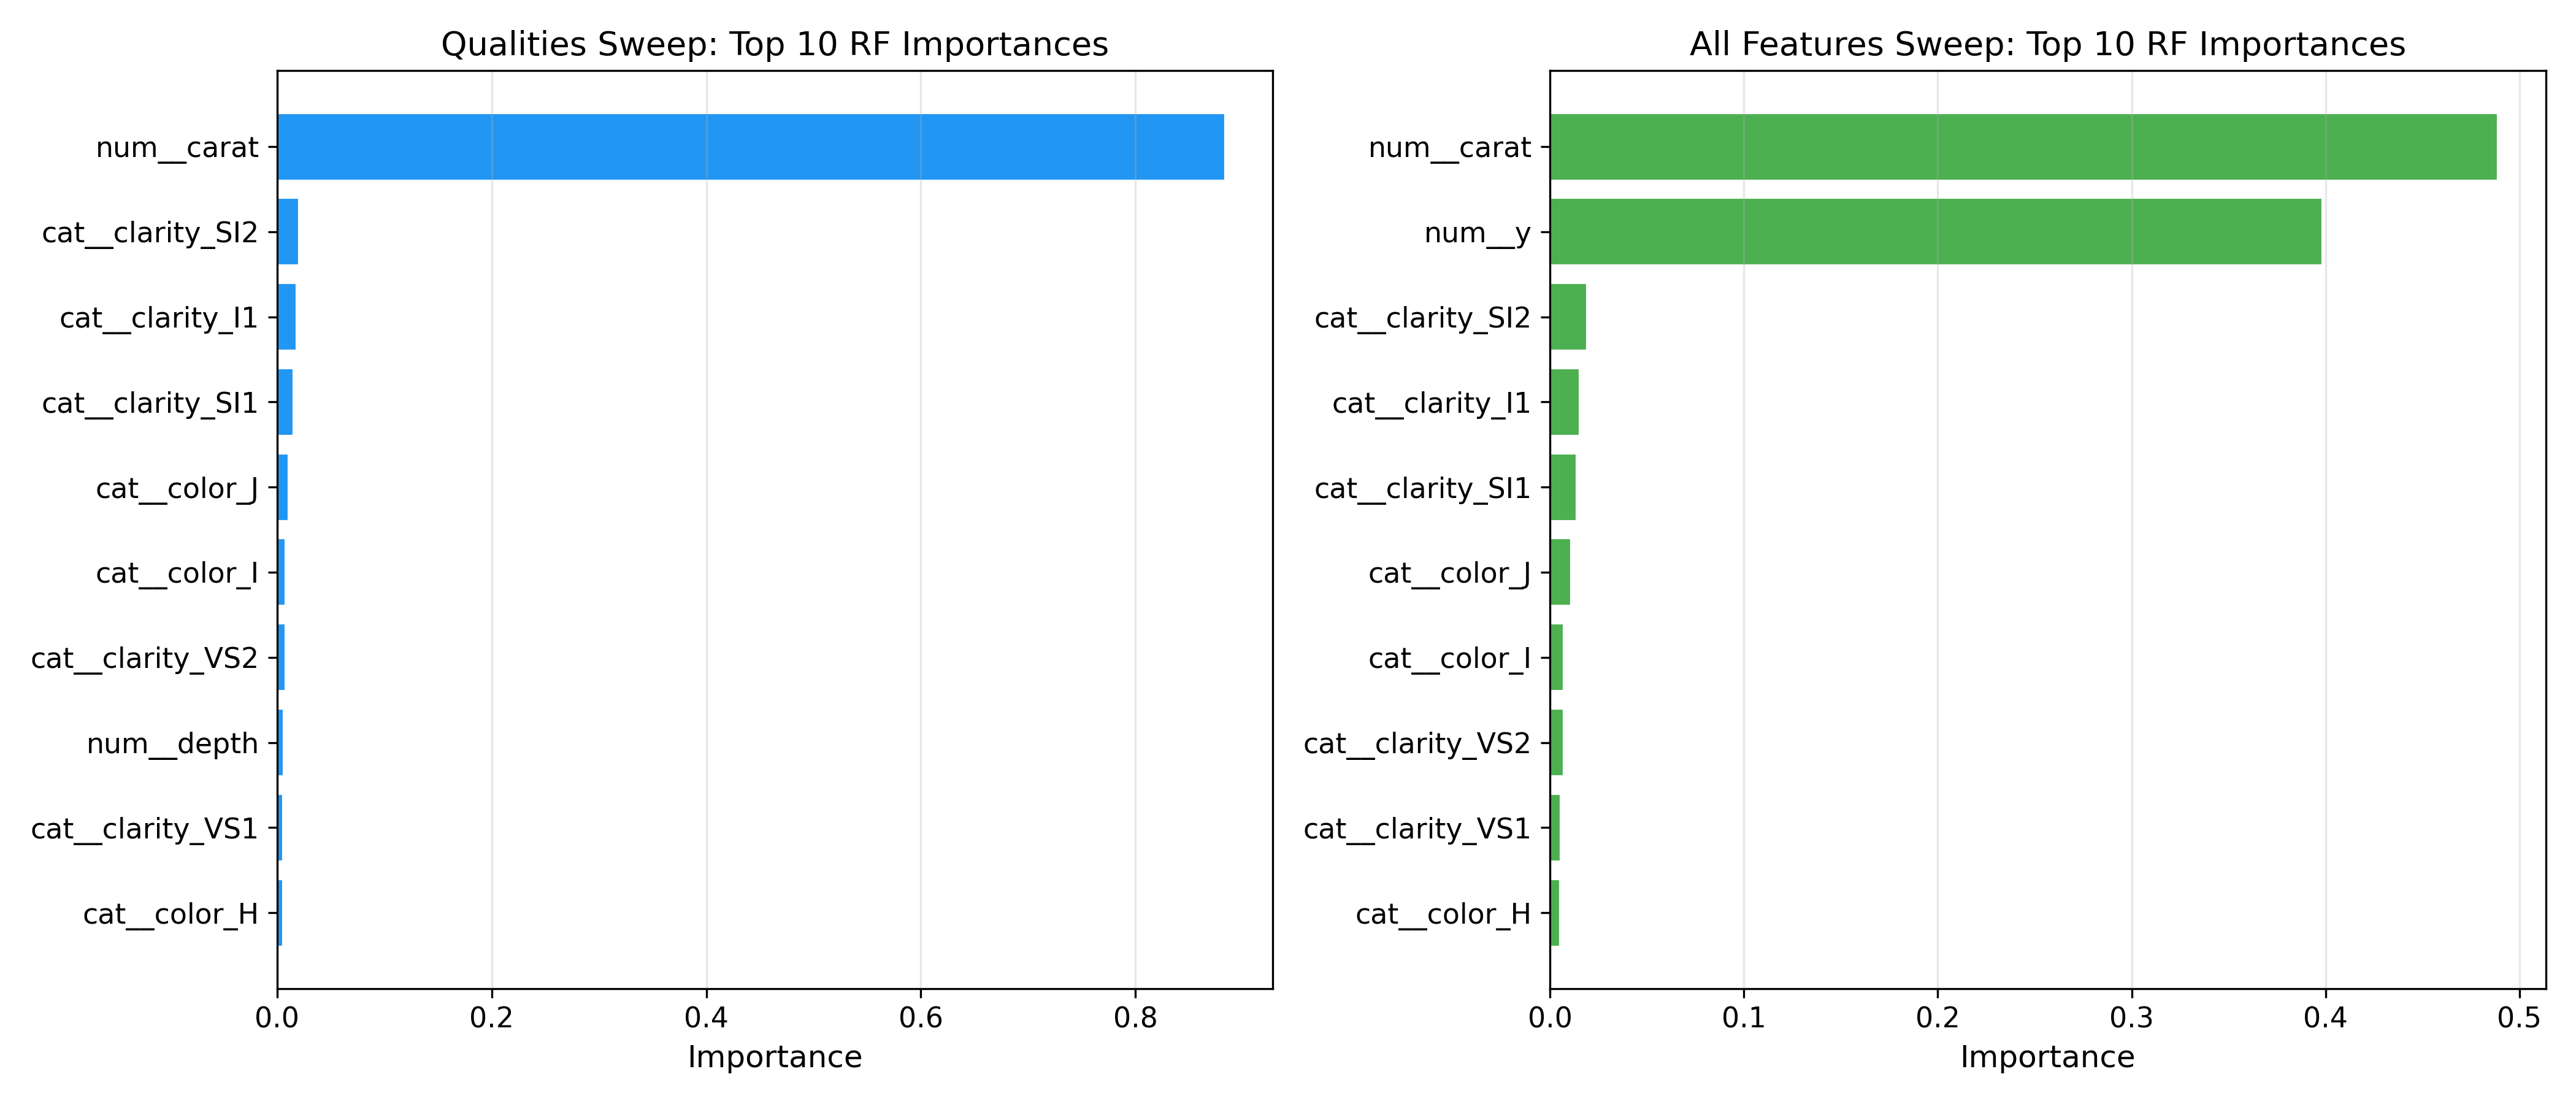
\includegraphics[width=\columnwidth]{plots/feature_importance_comparison.png}}
\caption{Top-10 Random Forest Gini importances. Left: qualities sweep (carat=88.4\%). Right: all-features sweep (carat=48.9\%, y=39.9\%).}
\label{fig:feature_imp}
\end{figure}

\subsubsection{Ablation Importance}

Leave-one-out ablation provides a complementary view of feature importance by measuring how much wMAPE degrades when each feature is removed. Fig.~\ref{fig:ablation} reveals a striking contrast with Gini importance.

\begin{figure}[htbp]
\centerline{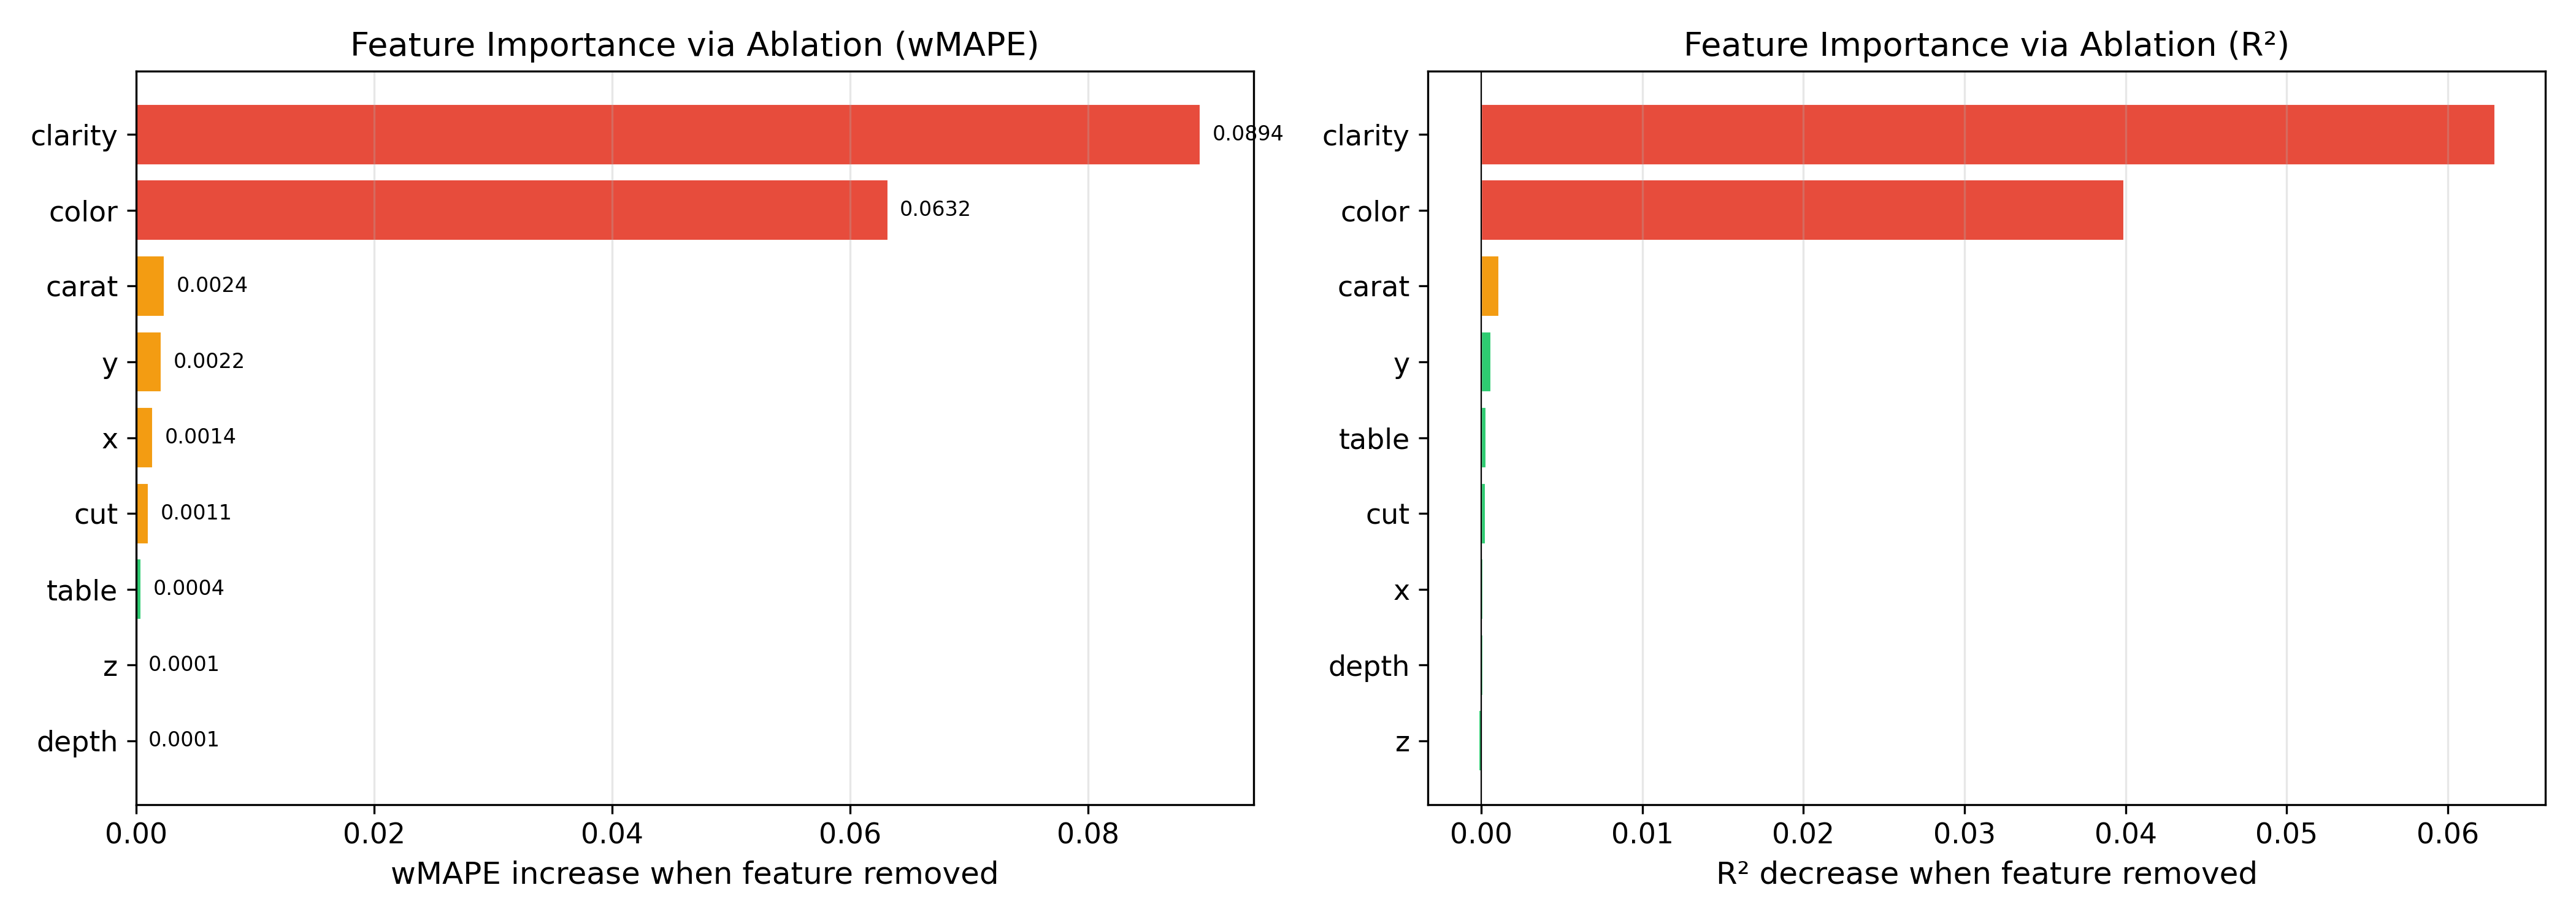
\includegraphics[width=\columnwidth]{plots/ablation_importance.png}}
\caption{Feature importance via leave-one-out ablation in the all-features sweep. Left: wMAPE increase upon removal. Right: $R^2$ decrease. Clarity and color are the most irreplaceable features despite modest Gini importance.}
\label{fig:ablation}
\end{figure}

\textbf{Clarity} causes the largest wMAPE increase when removed ($+0.089$, from 0.070 to 0.159), followed by \textbf{color} ($+0.063$). In contrast, \textbf{carat}---which dominates Gini importance at 88.4\%---has an ablation impact of only $+0.002$ because dimensions (\texttt{x}, \texttt{y}, \texttt{z}) serve as effective proxies for weight. This demonstrates that Gini importance measures how often a feature is used for splitting, not how irreplaceable its information is.

\subsection{Generalization and Overfitting}

Fig.~\ref{fig:train_val_test} compares train, validation, and test metrics for the best RF model from each sweep. Validation and test wMAPE are closely aligned across all sweeps (within 0.003), confirming robust generalization.

\begin{figure}[htbp]
\centerline{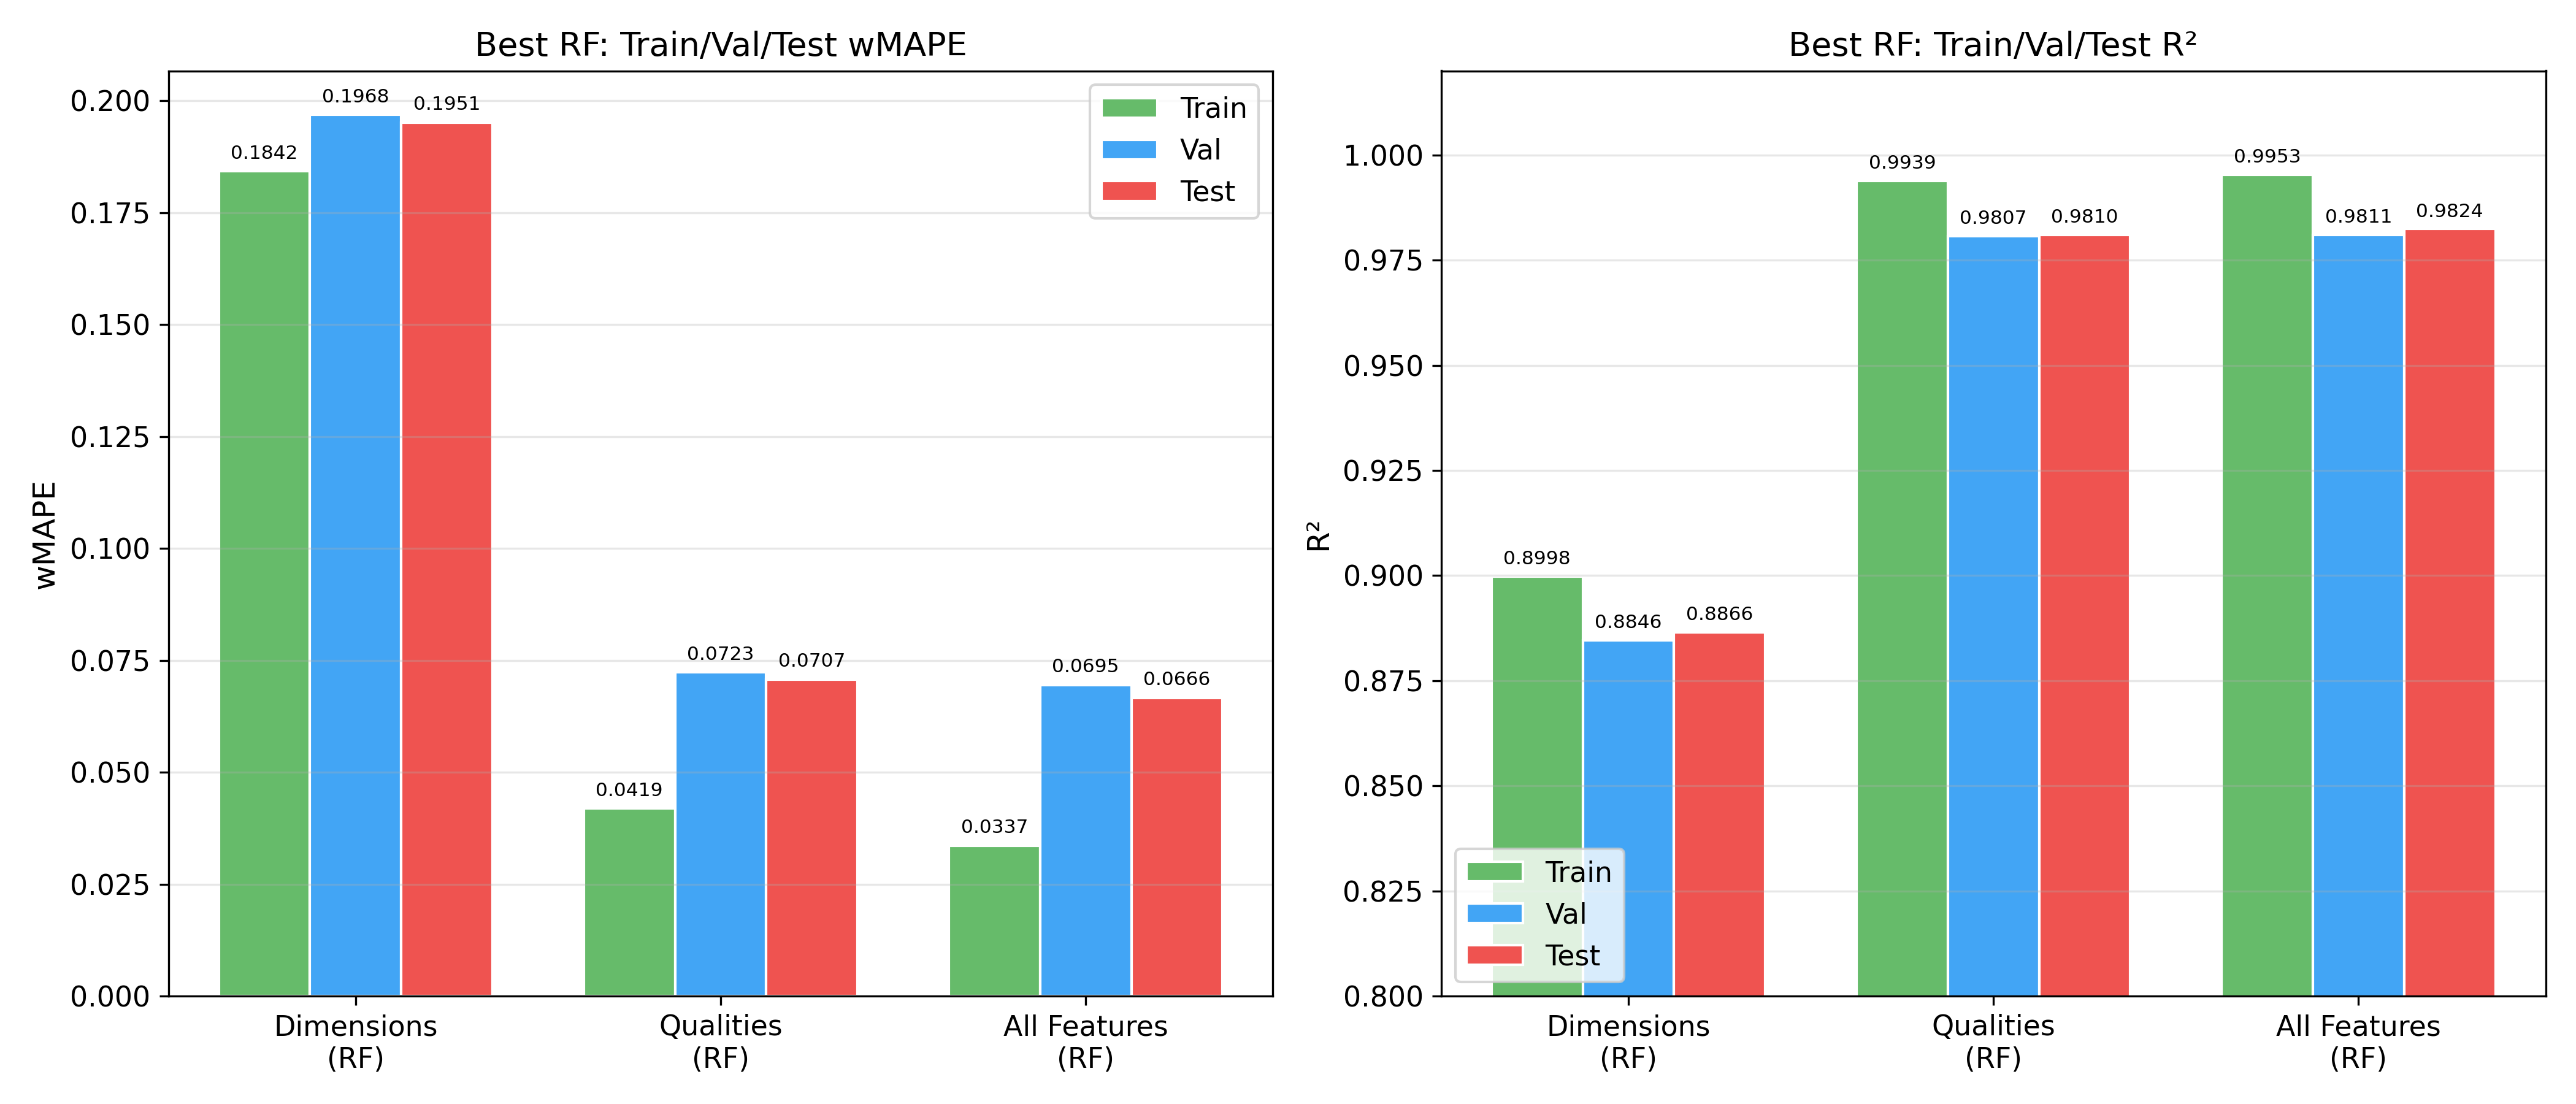
\includegraphics[width=\columnwidth]{plots/train_val_test_comparison.png}}
\caption{Train/validation/test wMAPE and $R^2$ for best RF models. The train-validation gap grows with feature richness (0.013 for dimensions, 0.036 for all features) but validation and test are consistently aligned.}
\label{fig:train_val_test}
\end{figure}

The train--validation wMAPE gap increases with model complexity: 0.013 for dimensions, 0.030 for qualities, and 0.036 for all features. This indicates mild overfitting to the richer feature spaces, but the consistent val--test alignment suggests the validation set provides reliable model selection.

\section{Discussion}

\subsection{The Primacy of Quality Attributes}

Our results demonstrate that quality attributes---particularly carat, clarity, and color---are the primary drivers of diamond prices. The qualities-only model achieves 96.1\% of the all-features model's performance (wMAPE 0.0723 vs.\ 0.0695), while dimensions alone capture only 35.3\% of the achievable accuracy improvement over a baseline. This aligns with gem industry practice, where pricing is fundamentally driven by the 4Cs rather than raw physical measurements~\cite{b1}.

\subsection{Redundancy Between Carat and Dimensions}

The ablation study reveals that carat weight is largely redundant with physical dimensions. Carat is a measure of weight, and for round-cut diamonds, weight is deterministically related to volume ($\propto x \cdot y \cdot z$). When both are available, the model can use either; removing one costs only $+0.002$ wMAPE. This redundancy inflates carat's Gini importance by making it a convenient split feature, even though its unique information contribution is small.

\subsection{Irreplaceability of Clarity and Color}

Clarity and color provide information about internal inclusions and light absorption that cannot be inferred from physical measurements. Their ablation impacts ($+0.089$ and $+0.063$ wMAPE) are 37$\times$ and 26$\times$ larger than carat's, respectively. This finding has practical implications: a price prediction system must include grading attributes; physical measurements alone are insufficient regardless of model sophistication.

\subsection{Nonlinearity of Diamond Pricing}

The consistent 2.7$\times$ gap between ElasticNet and RFR on the qualities sweep (wMAPE 0.197 vs.\ 0.072) demonstrates that diamond pricing involves strongly nonlinear relationships. The price--carat relationship is approximately polynomial (price $\propto$ carat$^{1.5}$ to carat$^2$), and categorical interactions (e.g., a VVS1-D diamond commands a disproportionate premium) cannot be captured by additive linear models. Tree-based ensembles naturally model these interactions through recursive partitioning.

\subsection{Curse of Dimensionality for KNN}

KNN performs comparably to RFR in the low-dimensional space (3 features: wMAPE 0.197 vs.\ 0.197) but deteriorates significantly with more features (9 features: 0.086 vs.\ 0.070). One-hot encoding of categoricals expands the effective dimensionality to 26, creating a sparse space where distance metrics become less meaningful. This is a well-known limitation of instance-based methods in high dimensions~\cite{b8}.

\subsection{Hyperparameter Heuristics for Future Runs}

Based on the parameter interaction analysis (Figs.~\ref{fig:nest_by_leaf}--\ref{fig:marginal}), we recommend the following heuristics for a follow-up sweep targeting even lower wMAPE:

\begin{itemize}
\item \textbf{Random Forest}: Fix \texttt{min\_samples\_leaf}$=1$--$2$ and \texttt{max\_depth}$\ge 20$ (or unlimited), then concentrate the grid on \texttt{n\_estimators}$\in \{500, 800, 1200, 1600\}$ to probe whether additional trees continue to reduce variance. The three-way heatmap (Fig.~\ref{fig:3way}) shows the current best region has not fully plateaued at 800 trees with unlimited depth.
\item \textbf{KNN}: Use distance weighting and sweep \texttt{n\_neighbors} $\in \{3, 5, 7\}$ for the high-dimensional all-features case.
\item \textbf{ElasticNet}: Fix \texttt{alpha}$\le 0.3$ and \texttt{l1\_ratio}$\in [0.3, 0.6]$; finer tuning is unlikely to close the gap with RF.
\item \textbf{General}: The top-vs-bottom analysis (Fig.~\ref{fig:topbot}) confirms that \texttt{max\_depth} is the most impactful RF parameter. Any new sweep should allocate most of its budget to combinations with \texttt{max\_depth}$\ge 20$.
\end{itemize}

\section{Conclusion}

We conducted a comprehensive evaluation of 9,798 model configurations for diamond price prediction across three feature sets. Key findings:

\begin{enumerate}
\item \textbf{Random Forest consistently achieves the best performance}, with a best wMAPE of 0.0695 ($R^2=0.981$), outperforming KNN by 19.3\% and ElasticNet by 63.0\%.
\item \textbf{Quality features dominate}: carat, cut, color, clarity, depth, and table alone achieve wMAPE 0.0723, only 3.9\% worse than using all 9 features.
\item \textbf{Ablation importance diverges from Gini importance}: clarity and color are the most irreplaceable features, while carat---despite 88\% Gini importance---is largely redundant with physical dimensions.
\item \textbf{Nonlinear models are essential}: ElasticNet achieves at best 0.188 wMAPE, confirming that diamond pricing involves complex, nonlinear interactions.
\item \textbf{Optimal RF hyperparameters scale with feature complexity}: max\_depth should increase from 10 to unlimited as features grow from 3 to 9.
\end{enumerate}

\ifdefined\IncludePartialRun
An exploratory partial run with a 5-feature subset and extended grid achieved best val wMAPE \LocalBestWmapeVal\ ($R^2$ = \LocalBestRtwoVal), confirming that the all-features sweep remains the best reference for deployment.
\fi
Future work should explore gradient boosting (XGBoost, LightGBM) for potential further gains, log-price transformation to improve accuracy on high-value diamonds, and stratified evaluation by price range to understand where model errors concentrate.

\begin{thebibliography}{00}
\bibitem{b1} Gemological Institute of America, ``Diamond Quality Factors,'' GIA 4Cs of Diamond Quality, 2024.
\bibitem{b2} Y. Chu, ``Predicting diamond prices using linear regression,'' \textit{Journal of Statistics Education}, vol. 9, no. 3, 2001.
\bibitem{b3} S. Agrawal and A. Kumar, ``Diamond price prediction using machine learning,'' in \textit{Proc. Int. Conf. on Computing and Communication}, pp. 1--5, 2020.
\bibitem{b4} M. Singh and R. Sharma, ``Ensemble methods for gemstone price estimation,'' \textit{Applied Intelligence}, vol. 52, pp. 4521--4535, 2022.
\bibitem{b5} H. Wickham, ``ggplot2: Elegant Graphics for Data Analysis,'' Springer-Verlag New York, 2016. (Diamonds dataset.)
\bibitem{b6} L. Breiman, ``Random forests,'' \textit{Machine Learning}, vol. 45, no. 1, pp. 5--32, 2001.
\bibitem{b7} H. Zou and T. Hastie, ``Regularization and variable selection via the elastic net,'' \textit{Journal of the Royal Statistical Society: Series B}, vol. 67, no. 2, pp. 301--320, 2005.
\bibitem{b8} R. E. Bellman, \textit{Adaptive Control Processes: A Guided Tour}. Princeton University Press, 1961.
\end{thebibliography}

\end{document}
